% First comes an example EPS file -- just ignore it and
% proceed on the \documentclass line
% your LaTeX will extract the file if required
\begin{filecontents*}{example.eps}
%!PS-Adobe-3.0 EPSF-3.0
%%BoundingBox: 19 19 221 221
%%CreationDate: Mon Sep 29 1997
%%Creator: programmed by hand (JK)
%%EndComments
gsave
newpath
  20 20 moveto
  20 220 lineto
  220 220 lineto
  220 20 lineto
closepath
2 setlinewidth
gsave
  .4 setgray fill
grestore
stroke
grestore
\end{filecontents*}



\RequirePackage{fix-cm}

\documentclass[smallextended]{./springer/svjour3}       % onecolumn (second format)

\smartqed  % flush right qed marks, e.g. at end of proof

\usepackage{amsmath}
\usepackage{amsfonts}

% Russian-specific packages
%--------------------------------------
\usepackage[T2A]{fontenc}
\usepackage[utf8]{inputenc}
\usepackage[russian]{babel}
%--------------------------------------

% Asymptote for pictures
%--------------------------------------
\usepackage{asymptote} %% comes with options inline and attach
%--------------------------------------

% graphicx for graphs
%--------------------------------------
\usepackage{graphicx}
% \usepackage{subfig}
\graphicspath{
    {./pic/,./asy/}
}
%--------------------------------------

% subcaption for many figures under one big caption
% each having its own small caption
%--------------------------------------
\usepackage{caption}
\usepackage{subcaption}
%--------------------------------------

\newtheorem{stmt}{Утверждение}
\newtheorem{prblm}{Затруднение}

% --------------------------------------------------------------
% ТИТУЛЬНЫЙ ЛИСТ И АННОТАЦИЯ
% --------------------------------------------------------------

\begin{document}

\title{Движение симметричного экипажа на омни-колесах\\с массивными роликами}
\subtitle{Уравнения движения и сравнение со случаем без роликов}

\author{Герасимов К.В. \and
        Зобова А.А
}

\institute{Кафедра теоретической механики и мехатроники\\
Механико-математический факультет\\
МГУ им. М.В. Ломоносова \at
              Москва\\
              Тел.: (495) 939-36-81\\
              \email{kiriger@gmail.com, azobova@gmail.com}
}

\maketitle

\begin{abstract}
В статье рассматривается модель экипажа с роликонесущими колесами, учитывающая массы роликов, оценивается отличие в уравнениях движения от постановки без роликов и приводятся результаты численного решения для некоторых движений.

Ключевые слова: омниколеса \and роликонесущие колеса \and лаконичная форма уравнений движения Я.В. Татаринова

\end{abstract}

\newpage

% --------------------------------------------------------------
% ВВЕДЕНИЕ
% --------------------------------------------------------------

\section{Введение}

% все рассматривают экипажи с колесами без роликов, налагая такие-то связи, и задачи хорошо исследуются (в таких-то работах)
Задачи динамики систем тел, связянные с роликонесущими колесами и экипажами, использующими их, часто становятся объектами исследований, однако, как правило, либо рассматриваются упрощенные модели, пренебрегающие инерцией и формой роликов \cite{ZobovaTatarinov, Martynenko, Borisov}, либо используются формализмы для построения численных моделей систем тел, скрывающие явный вид уравнений движения \cite{KosenkoGerasimov, MaybeTobolar, Others}.

Цель настоящей работы -- получение уравнений движения по инерции экипажа с омни-колесами с массивными роликами в неголономной постановке с помощью подхода \cite{Tatarinov} и сравнение поведения такой системы с поведением системы без роликов \cite{Zobova2011}.

% массы роликов могут достигать такой-то доли от массы всего колеса (ссылки!), и потому имеет смысл рассмотреть полную постановку

% ряд движений исчезнет, изчезнет первый интеграл и вообще мало ли что - про это не буду писать, т.к. движения не исчезли, и мы вообще-то строго не проверяли, что тут с интегралами.

% покажем, что уравнения отличаются наличием слагаемых порядка собственного момента инерции ролика
% возникнут сложности с переходом между роликами, преодолеем их, введя некоторые упрощения.
В статье показаны отличия в уравнениях движения, возникающие при добавлении роликов -- это явная зависимость правых частей от углов поворота колес (и, следовательно, необходимость добавить уравнения связей для получения полной системы) и наличие слагаемых порядка собственного момента инерции ролика. Также обсуждается смена контакта роликов и возникающие в связи с ней разрывы в правых частях уравнений движения, которые здесь устраняются путем введения дополнительных предположений о характере движения роликов. В заключение приводятся результаты численного решения полученных уравнений движения для симметричной трехколесной конфигурации экипажа и основных вариантов начальных условий в постановках с роликами и без.



% --------------------------------------------------------------
% ПОСТАНОВКА ЗАДАЧИ
% --------------------------------------------------------------

\section{Постановка задачи}

\begin{figure}
    \minipage{0.5\textwidth}
        \centering
        \asyinclude{./asy/pic_cart.asy}
        \caption{Экипаж}
        \label{fig:vehicle}
    \endminipage
    \minipage{0.5\textwidth}
        \centering
        \asyinclude{./asy/pic_wheel.asy}
        \caption{Колесо}
        \label{fig:wheel}
    \endminipage
\end{figure}

Рассмотрим экипаж с омни-колесами, движущийся по инерции по неподвижной абсолютно шероховатой горизонтальной плоскости. Экипаж состоит из платформы и $N$ омни-колес, плоскости которых относительно платформы неподвижны. Каждое колесо может свободно вращаться относительно платформы вокруг собственной оси, расположенной горизонтально. Будем считать, что на каждом колесе установлено $n$ массивных роликов, так что оси роликов лежат в плоскостях колёс и направлены по касательной к границам дисков колес (см. рис.~\ref{fig:wheel}). Таким образом, система состоит из $N(n+1) + 1$ абсолютно твердых тел. 

Введем неподвижную систему отсчета так, что ось $OZ$ направлена вертикально вверх, а плоскость $OXY$ совпадает с опорной плоскостью.
Введем также подвижную систему отсчета $S\xi\eta Z$, жестко связанную с платформой экипажа так, что плоскость $S\xi\eta$ горизонтальна и содержит центры всех колес $P_i$. Будем считать, что оси колес лежат на лучах, соединяющих центр платформы $S$ и центры колес (см. рис.~\ref{fig:vehicle}), а расстояния от центров колес до $S$ одинаковы и равны $R$. Геометрию установки колес на платформе зададим углами $\alpha_i$ осями колес и осью $S\xi$
(см. рис.~\ref{fig:wheel}). Введем также орты, жестко связанные с дисками колес: пусть $\vec{n}_i = \vec{SP_i}/|\vec{SP_i}|$ -- единичный орт оси $i$-ого колеса, и орты $\vec{n}_i^\perp$ и $\vec{n}_i^z$, лежащие в плоскости диска колеса, так что вектор $\vec{n}_i^z$ вертикален при нулевом повороте колеса. Положения центров роликов на колесе определим углами $\kappa_j$ между ними и направлением, противоположным вектору $\vec{n}_i^z$. 

Положение экипажа будем задавать следующими координатами:
$x, y$ --- координаты точки $S$ на плоскости $OXY$, $\theta$ -- угол между $OX$ и $S\xi$ (угол курса),
$\chi_i$ ($i = 1\dots N$) -- углы поворота колес вокруг их осей, отсчитываемые против часовой стрелки, если смотреть с конца вектора $\vec{n}_i$, и $\phi_j$ -- углы поворота роликов вокруг их собственных осей.
Таким образом, вектор обобщенных координат имеет вид:
$$\vec{q} = (x, y, \theta, \left.\{\chi_i\}\right|_{i=1}^N , \left.\{\phi_k\}\right|_{k=1}^N, \phi_s)\in\mathbb{R}^{N(n+1) + 3}$$ 
Будем использовать обозначение $\phi_k$ для углов поворота роликов, находящихся в данный момент в контакте с опорной плоскостью, и $\phi_s$ для остальных --- ``cвободных'' --- роликов.

Будем считать, что проскальзывания между опорной плскостью и роликов в контакте не происходит, т.е.
скорости точек $C_i$ контакта равны нулю:
$$\vec{v}_{C_i} = 0,\quad i = 1\dots N.$$
Эти равенства дадут $2N$ независимых дифференциальных связей, следовательно, число степеней свободы системы равно $N(n-1) +3$.

Запишем уравнения связей и уравнения движения, используя следующие псевдоскорости
$$\nu = (\nu_1, \nu_2, \nu_3, \nu_s), \quad \vec{v}_S = R\nu_1\vec{e}_\xi + R\nu_2\vec{e}_\eta, \quad \nu_3 = \Lambda\dot{\theta},\quad \nu_s = \dot{\phi}_s$$
Их механический смысл таков: $\nu_1$, $\nu_2$ --- проекции скорости точки $S$ на оси $S\xi\eta$, связанные с платформой, $\nu_3$ --- с точностью до множителя угловая скорость платформы, $\nu_s$ --- угловые скорости свободных роликов.

К связям, налагаемым в случае модели омни-колеса без роликов \cite{Zobova2011}
$$ \dot{x} = R \nu_1\cos\theta-R\nu_2\sin\theta, \hspace{15pt} \dot{y} = R\nu_1\sin\theta+R\nu_2\cos\theta,$$
$$\dot{\theta} = \frac{\nu_3}{\Lambda}, \hspace{15pt} \dot{\chi}_i = \frac{R}{l}(\nu_1\sin\alpha_i - \nu_2\cos\alpha_i - \frac{\nu_3}{\Lambda}),$$
добавим связи для роликов, находящихся в контакте:
\begin{equation}\label{constraint_roller_contact}
\dot{\phi_k} = \frac{R}{l\cos\chi_k-r}(\nu_1\cos\alpha_k + \nu_2\sin\alpha_k)    
\end{equation}
и для свободных роликов:
$$\dot{\phi}_s = \nu_s.$$
Обратим внимание, что  знаменатель в (\ref{constraint_roller_contact}) есть расстояние от оси ролика до точки контакта: $\rho_k = l\cos\chi_k - r$, обращающееся в ноль на стыке роликов (см. рис.~\ref{fig:wheel}). Это обстоятельство приводит к неустранимым разрывам правых частей уравнений движения и будет рассмотрено отдельно ниже.

% --------------------------------------------------------------
% УРАВНЕНИЯ ДВИЖЕНИЯ
% --------------------------------------------------------------

\section{Уравнения движения}

Воспользуемся лаконичным методом получения уравнений движения для систем с дифференциальными связями, предложенным Я.В. Татариновым \cite{Tatarinov}:
\begin{equation}\label{Tatarinov}
    \frac{d}{dt}\frac{\partial L^{*}}{\partial \nu_\alpha}  + \{P_\alpha, L^{*}\} = \{P_\alpha, \nu_\mu P_\mu\}, 
\end{equation}
$$\nu_\mu P_\mu = \dot{q_i} p_i, \hspace{10pt} p_i = \frac{\partial L}{\partial \dot{q}_i},$$
где $P_\alpha, p_i$ -- формальные ``импульсы'', $L$ -- лагранжиан, $L^*$ -- он же с учетом связей, $\{\cdot, \cdot\}$ -- формальная скобка Пуассона.

Кинетическая энергия имеет вид:
$$ 2T = 2L = M\vec{v}_S^2 + I_S\dot{\theta}^2 + J\sum_i\dot{\chi}_i^2 + B\sum_{i,j}(\dot{\phi}_{ij}^2 + 2\dot{\theta}\sin(\kappa_j + \chi_i)\dot{\phi}_{ij}),$$
в котором, по сравнению со случаем без роликов, добавилось слагаемое, пропорциональное $B$ -- моменту инерции ролика относительно его оси вращения.

Также, изменились значения коэффициентов: полная масса системы -- $M = \mathring{M} + Nnm$, момент инерции всей системы относительно $SZ$ -- $I_S = \mathring{I_S} + Nn(\frac{A+B}{2} + mR^2 + \frac{mr^2}{2})$, момент инерции колеса (с роликами) относительно его оси $J = \mathring{J} + n(A + mr^2)$, где $\mathring{M}, \mathring{I_S}, \mathring{J}$ -- масса и моменты инерции системы и колес без учета роликов; $m$ -- масса ролика; $A$ -- момент инерции ролика относительно любой оси, перпендикулярной его оси собственного вращения и проходящей через его центр масс; $r$ -- радиус диска колеса (расстояние от центра колеса до центра ролика).

Лагранжиан с учетом связей имеет вид:
$$ 2L^{*} = \mathring{\nu}^T \mathring{V}^T \mathring{M} \mathring{V} \mathring{\nu} + $$
$$ + B\sum_{i}(
	\frac{(\nu_2\sin\alpha_i+\nu_1\cos\alpha_i)^2R^2}
	{\rho_i^2} +
	\frac{2R\nu_3(\nu_2\sin\alpha_i+\nu_1\cos\alpha_i)\sin\chi_i}
	{\rho_i\Lambda}
) + $$
$$+ B\sum_{i,j}(
	\frac{2\nu_3\nu_{3+ni+j}\sin(\kappa_j+\chi_i)}
	{\Lambda}
	+
	\nu_{3+ni+j}^2
)
$$
где $\frac{1}{2}\mathring{\nu}^T \mathring{V}^T \mathring{M} \mathring{V} \mathring{\nu} = \mathring{L}^{*}$ -- лагранжиан системы без роликов, матрицы кинетической энергии и связей для системы без роликов:
$$
\mathring{M} = diag(M, M, I_S, J...J),
\quad
\mathring{V} = \begin{bmatrix}
    R\cos\theta & -R\sin\theta & 0 \\
    R\sin\theta & R\cos\theta  & 0 \\
    0           & 0            & \frac{1}{\Lambda} \\
    \frac{R}{l}\sin\alpha_i & -\frac{R}{l}\cos\alpha_i & -\frac{R}{l\Lambda} \\
\end{bmatrix},
$$
$\nu_{3+nu+j} = \nu_s$ соответствуют свободным роликам.

% --------------------------------------------------------------
% ОТЛИЧИЯ ОТ СЛУЧАЯ БЕЗ РОЛИКОВ
% --------------------------------------------------------------

Таким образом, лагранжиан и ``импульсы'' отличаются от оных в случае без роликов аддитивными членами:
$$ L^{*} = \mathring{L}^{*} + BL^{*}_\Delta(\nu, \chi),$$
$$ P_\alpha = \mathring{P_\alpha}(\theta, p_x, p_y, p_\chi) + P_\Delta(p_{\phi_i}, \chi),$$
что для последних проверяется прямым подсчетом. Поэтому имеет место следующий факт.

\begin{stmt}
    Учет массы роликов приводит к появлению в правой части дифференциальных уравнений, описывающих динамику экипажа, слагаемых, пропорциональных собственному моменту инерции роликов $B$ и квадратично зависящих от псевдоскоростей. Эти новые слагаемые явно зависят от углов поворота колес $\chi_i$.
    $$\boldsymbol{A}\dot{\boldsymbol{\nu}} = \frac1\Lambda
    \left(
    \begin{array}{c}
         \nu_2\nu_3  \\
         -\nu_1\nu_3 \\
         0
    \end{array}
    \right) + B
     \left(
    \begin{array}{c}
         \boldsymbol{\nu}^T\boldsymbol{F}_1(\chi_i)\boldsymbol{\nu}  \\
         \boldsymbol{\nu}^T\boldsymbol{F}_2(\chi_i)\boldsymbol{\nu} \\
         \boldsymbol{\nu}^T\boldsymbol{F}_3(\chi_i)\boldsymbol{\nu}
    \end{array}
    \right),
    $$
    $$
    \dot{\chi}_i = \frac{R\sin\alpha_i}{l}\nu_1 - \frac{R\cos(\alpha_i)}{l}\nu_2 - \frac{R}{l\Lambda}\nu_3, \quad i = 1..N,
    $$
    $$
    \Lambda\dot{\nu}_{ni+j} = -\dot{\nu}_3\sin(\chi_i+\kappa_j) - \dot{\chi_i}\nu_3\cos(\chi_i+\kappa_j), \quad j = 2..n.
    $$
\end{stmt}

Для доказательства достаточно рассмотреть по очереди члены в лаконичной форме уравнений \ref{Tatarinov}:

$$ \frac{d}{dt}\frac{\partial }{\partial \nu_\alpha}(L^{*} - \mathring{L^{*}}) = B\frac{d}{dt}\frac{\partial}{\partial \nu_\alpha}L^{*}_\Delta(\nu, \chi), $$
$$ \{P_\alpha, L^{*}\} - \{\mathring{P}_\alpha, \mathring{L}^{*}\} = B\{ P_\alpha, L^{*}_\Delta(\nu, \chi) \} $$
$$\{P_\alpha, P_\mu\} - \{\mathring{P}_\alpha, \mathring{P}_\mu\} = B\frac{R^2}{\Lambda}\sum_i\frac{f_\alpha(\nu, \chi)}{\rho^2_i}(\frac{R}{\rho_i}(\nu_1\cos\alpha_i + \nu_2\sin\alpha_i) + \frac{\sin\chi_i}{\Lambda}\nu_3).$$


% --------------------------------------------------------------
% ПЕРЕХОД МЕЖДУ РОЛИКАМИ
% --------------------------------------------------------------

\section{Переход между роликами}

\begin{figure}
    \minipage{0.5\textwidth}
        \centering
        \asyinclude{./asy/pic_overlap.asy}
        \caption{Ролики перекрываются}
        \label{fig:overlap}
    \endminipage
    \minipage{0.5\textwidth}
        \centering
        \asyinclude{./asy/pic_change.asy}
        \caption{Переход между роликами}
        \label{fig:change}
    \endminipage
\end{figure}

Чтобы исследовать поведение системы, необходимо описать переход колеса с одного ролика на другой. Здесь мы немедленно сталкиваемся с затруднением, указанным выше: уравнения движения вырождаются на стыках роликов, т.к. квадратичные формы $\boldsymbol{F}_i$ терпят разрыв 2ого рода из-за выражений $\rho_i = l\cos\chi_i-r$ в знаменателе.

Заметим, что в технических реализациях роликонесущих колес ситуация $\rho_i = 0$ никогда не имеет места, т.к. концы роликов усекаются (ФОТО?) (в частности, потому что оси роликов в реальных системах имеют ненулевую толщину и должны быть закреплены в колесах), а чтобы граница проекции колеса на его плоскость оставалась окружностью, ролики располагают либо под углом (как в меканум-колесах, (ФОТО?)), либо в два или больше рядов (ФОТО?). Подобные расположения приводят, впрочем, к скачкам точек контакта в моменты смены роликов, что также создаст разрывы в правых частях уравнений.

Поэтому для начала, мы усечем ролики (см. рис.~\ref{fig:overlap}), но оставим их оси в одной плоскости, допуская пересечение тел роликов в пространстве и пренебрегая им.

Кроме этого, при смене контакта происходит мгновенное наложение связи на вновь вошедший в контакт ролик (и снятие её с освободившегося). В настоящей работе, будем считать, что ролик, входящий в контакт, мгновенно оказывается закручен до той же угловой скорости, до которой закручен освобождающийся ролик, а последний мгновенно прекратит собственное вращение. Таким образом, мы будем рассматривать только движение роликов, находящихся в контакте.

Для этого, отбросим уравнения
$$
\Lambda\dot{\nu}_{ni+j} = -\dot{\nu}_3\sin(\chi_i+\kappa_j) - \dot{\chi_i}\nu_3\cos(\chi_i+\kappa_j), \quad i = 1..n, j = 2..n,
$$
описывающие движение свободных роликов, и при переходе ($\chi_i = \chi_i^+$) сохраним значения $\nu_1$, $\nu_2$, 
$\nu_3$, $\chi_i$ заменим с $\chi_i^+$ на $\chi_i^-$ (см. рис.~\ref{fig:change}), а $\dot\chi_i$ пересчитаем по уравнениям связей.

% --------------------------------------------------------------
% ЧИСЛЕННОЕ РЕШЕНИЕ - ПРИМЕРЫ
% --------------------------------------------------------------

\section{Примеры движений}

% \begin{figure}
    \centering
    \begin{subfigure}[t]{0.3\textwidth}
        \centering
        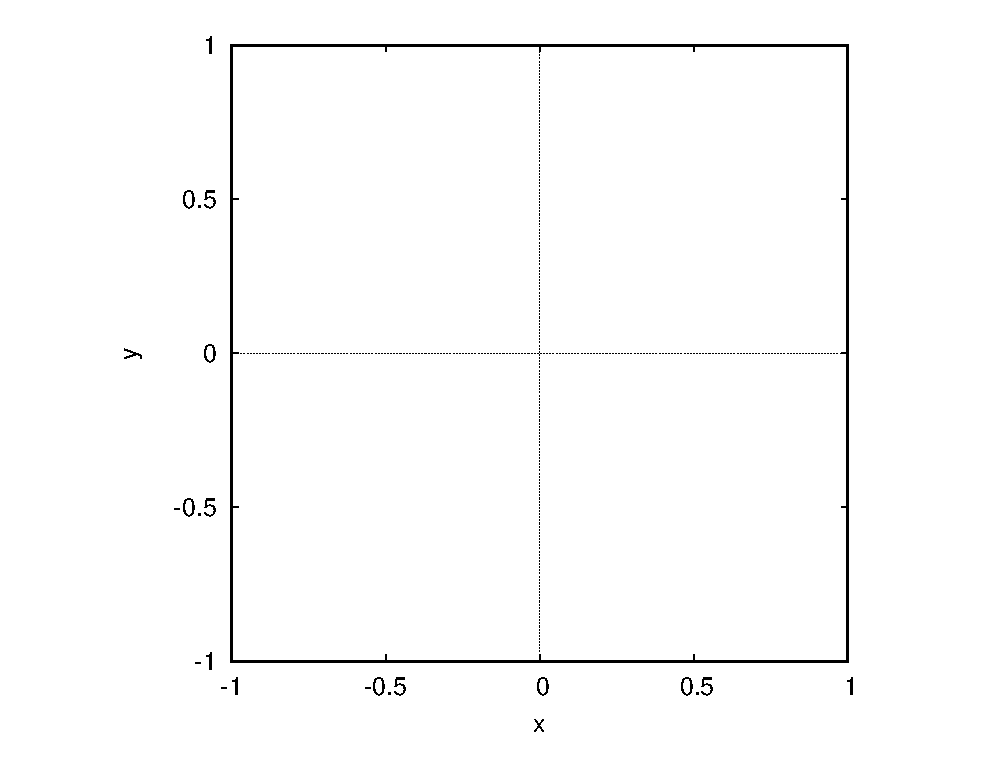
\includegraphics[width=\linewidth, height=30mm]{pic/_old_sol__0_0_1__0__10__1e2_trajectory}
        \caption{Траектория $X, Y$}
        \label{fig:_old_sol__0_0_1__0__10__1e2_trajectory}
    \end{subfigure}
    \begin{subfigure}[t]{0.3\textwidth}
        \centering
        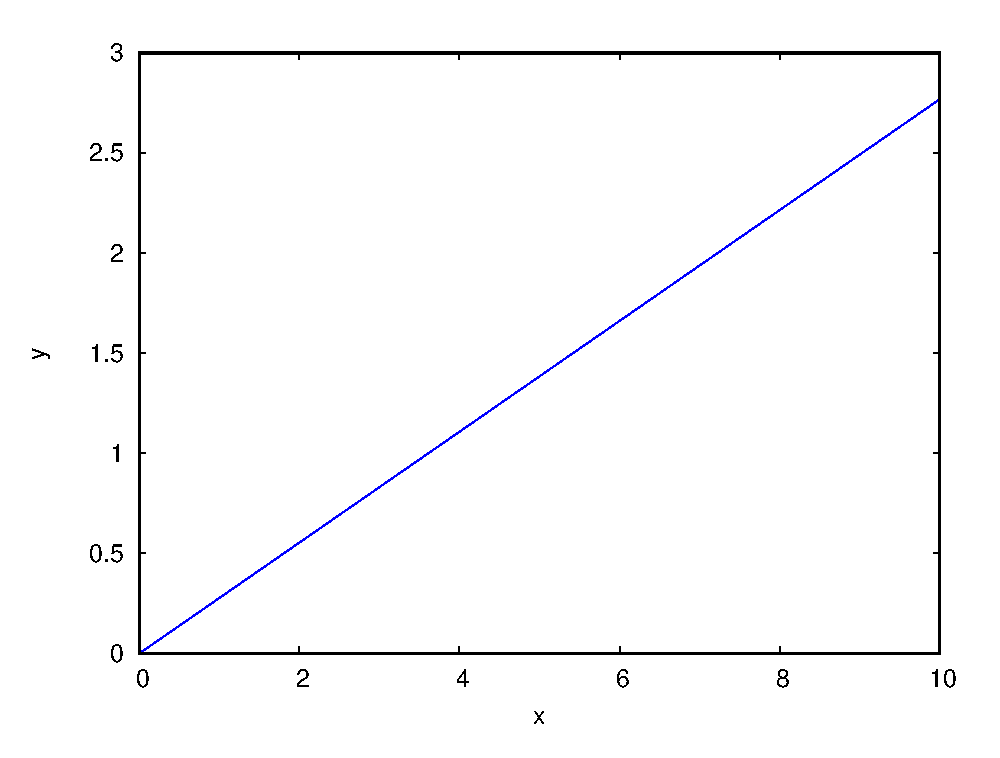
\includegraphics[width=\linewidth, height=30mm]{pic/_old_sol__0_0_1__0__10__1e2_theta}
        \caption{$\theta(t)$}
        \label{fig:_old_sol__0_0_1__0__10__1e2_theta}
    \end{subfigure}
    \vspace{12pt}
    
    \begin{subfigure}[t]{0.3\textwidth}
        \centering
        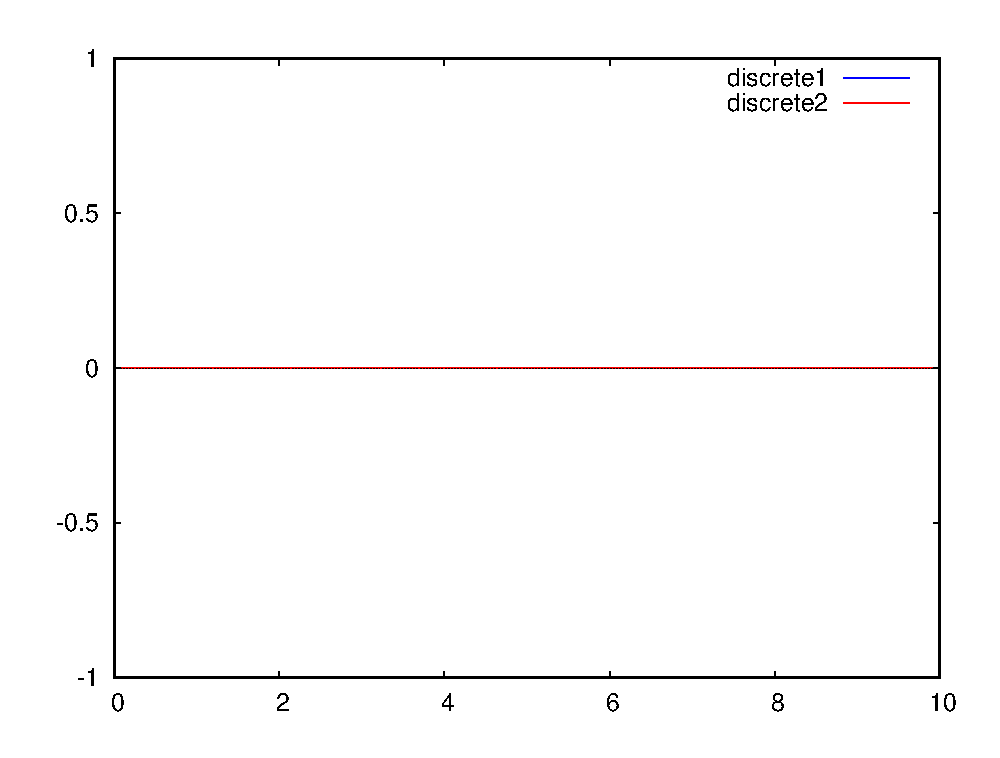
\includegraphics[width=\linewidth, height=30mm]{pic/_old_sol__0_0_1__0__10__1e2_nu12}
        \caption{$\nu_1(t), \nu_2(t)$}
        \label{fig:_old_sol__0_0_1__0__10__1e2_nu12}    
    \end{subfigure}
    \hfill
    \begin{subfigure}[t]{0.3\textwidth}
        \centering
        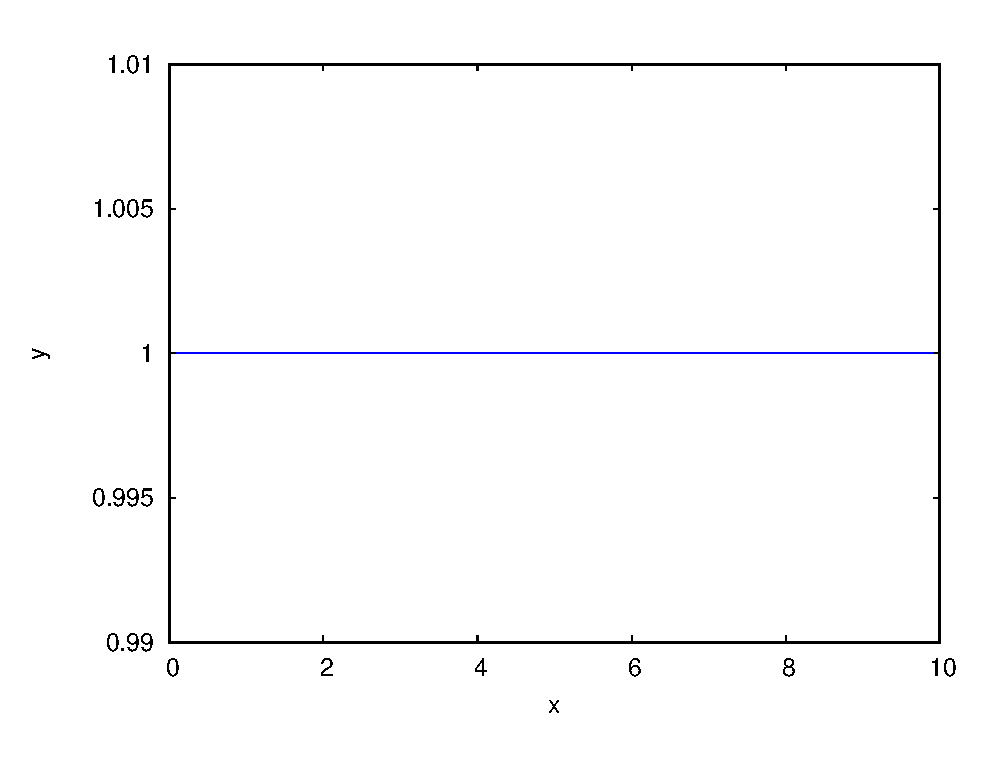
\includegraphics[width=\linewidth, height=30mm]{pic/_old_sol__0_0_1__0__10__1e2_nu3} \\
        \caption{$\nu_3(t)$}
        \label{fig:_old_sol__0_0_1__0__10__1e2_nu3}
    \end{subfigure}
    \hfill
    \begin{subfigure}[t]{0.3\textwidth}
        \centering
        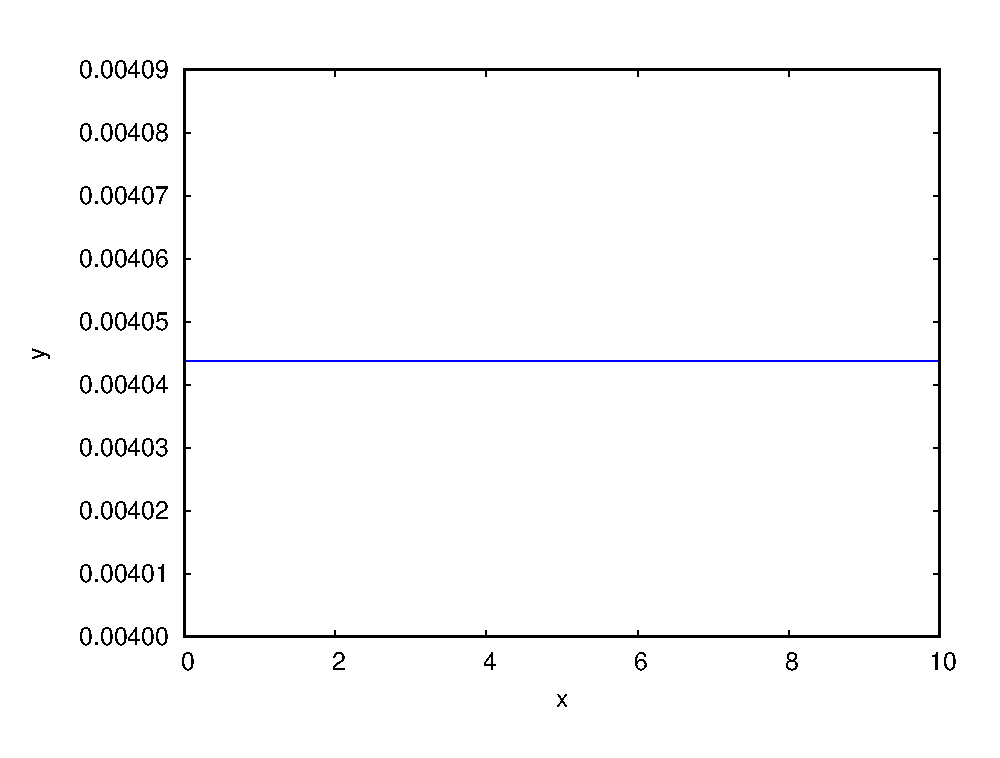
\includegraphics[width=\linewidth, height=30mm]{pic/_old_sol__0_0_1__0__10__1e2_kin_en}
        \caption{Кинетическая энергия}
        \label{fig:_old_sol__0_0_1__0__10__1e2_kin_en}
    \end{subfigure}
    
    \caption{Экипаж без роликов. Вращение вокруг своей оси ($\nu_{1,2}(0) = 0, \nu_3 = 1$). Центр экипажа неподвижен, скорость вращения и энергия постоянны.}
    \label{fig:old_selfrot}
\end{figure}

% \begin{figure}
    \centering

    % \begin{subfigure}[t]{0.3\textwidth}
    %     \centering
    %     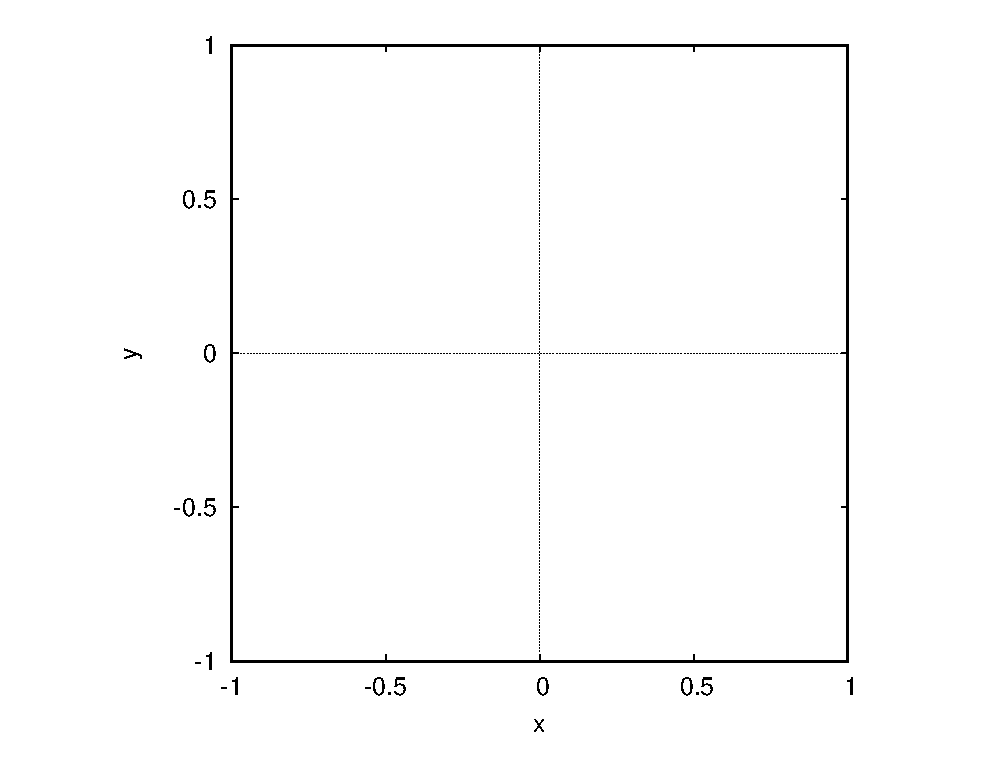
\includegraphics[width=\linewidth, height=30mm]{pic/_sol__0_0_1__0__10__1e2_trajectory}
    %     \caption{Траектория $X, Y$}
    %     \label{fig:_sol__0_0_1__0__10__1e2_trajectory}
    % \end{subfigure}
    % \begin{subfigure}[t]{0.3\textwidth}
    %     \centering
    %     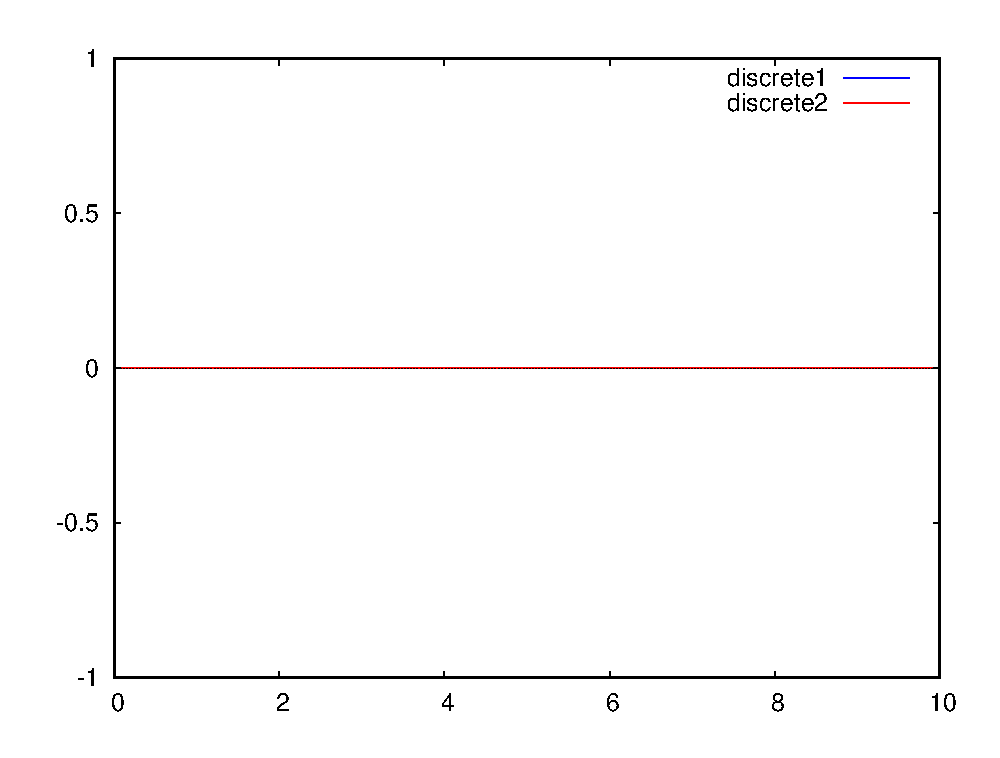
\includegraphics[width=\linewidth, height=30mm]{pic/_sol__0_0_1__0__10__1e2_nu12}
    %     \caption{$\nu_1(t), \nu_2(t)$}
    %     \label{fig:_sol__0_0_1__0__10__1e2_nu12}    
    % \end{subfigure}
    
    % \begin{subfigure}[t]{0.3\textwidth}
    %     \centering
    %     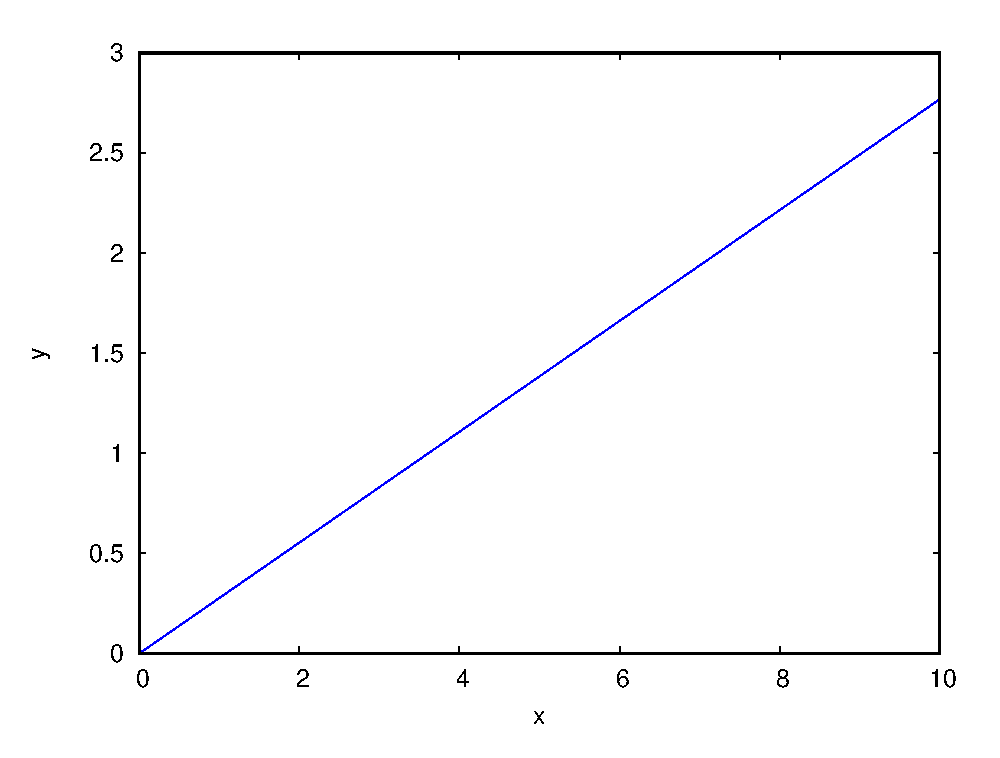
\includegraphics[width=\linewidth, height=30mm]{pic/_sol__0_0_1__0__10__1e2_theta}
    %     \caption{$\theta(t)$}
    %     \label{fig:_sol__0_0_1__0__10__1e2_theta}
    % \end{subfigure}
    % \vspace{12pt}
    
    % \begin{subfigure}[t]{0.3\textwidth}
    %     \centering
    %     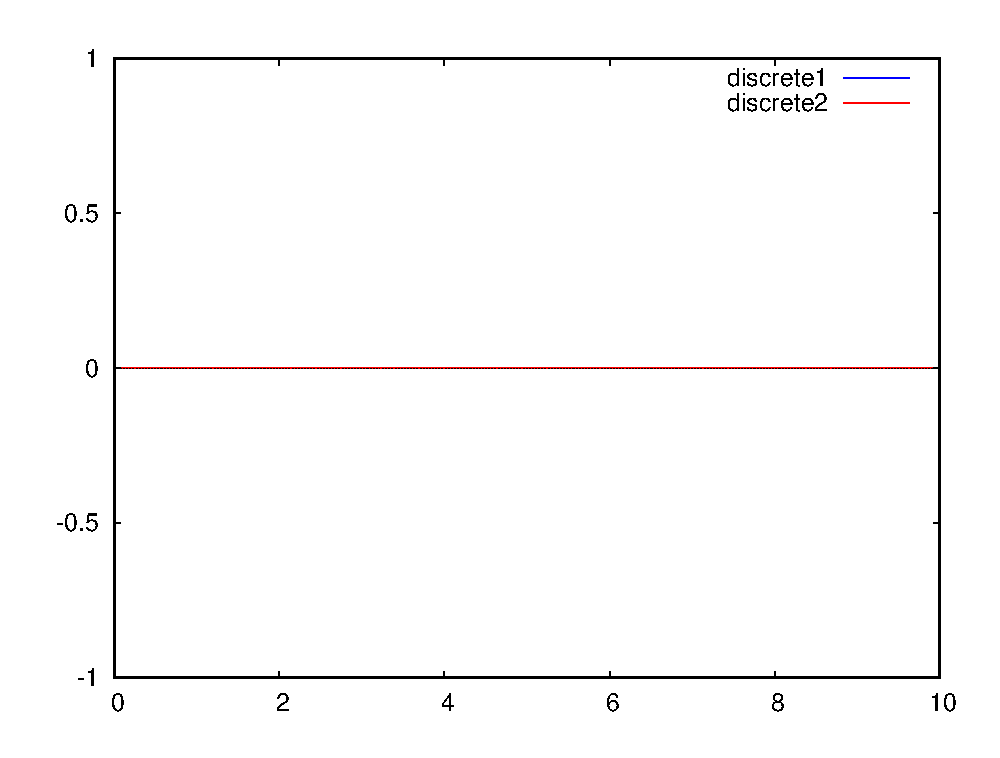
\includegraphics[width=\linewidth, height=30mm]{pic/_sol__0_0_1__0__10__1e2_nu12}
    %     \caption{$\nu_1(t), \nu_2(t)$}
    %     \label{fig:_sol__0_0_1__0__10__1e2_nu12}    
    % \end{subfigure}
    % \hfill
    % \begin{subfigure}[t]{0.3\textwidth}
    %     \centering
    %     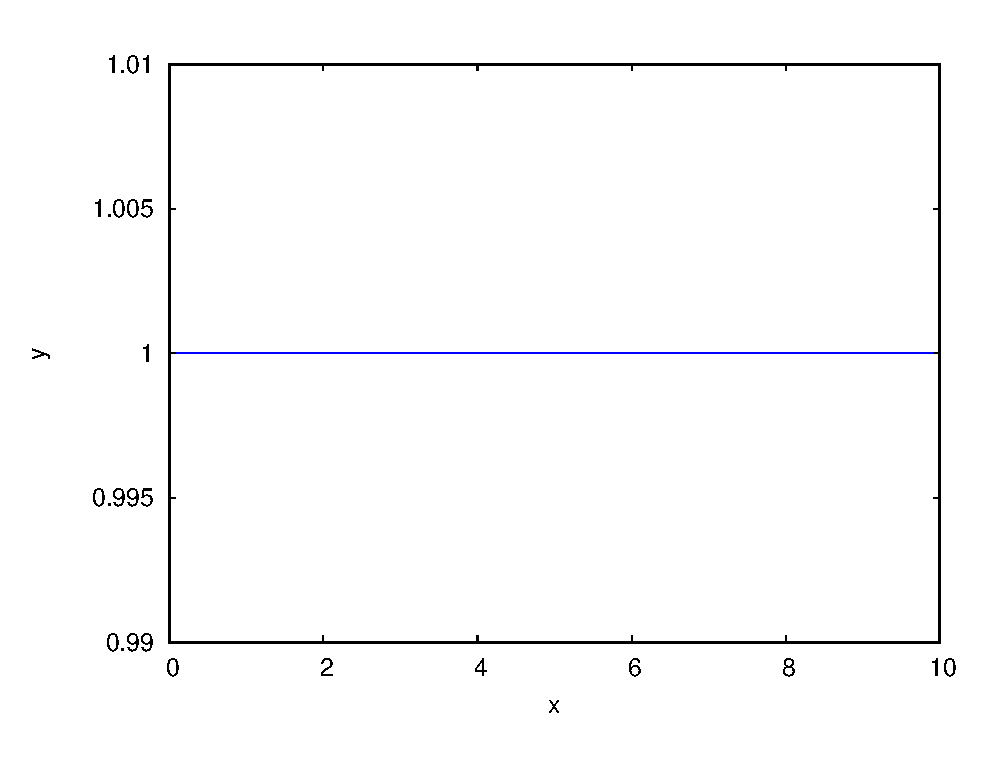
\includegraphics[width=\linewidth, height=30mm]{pic/_sol__0_0_1__0__10__1e2_nu3} \\
    %     \caption{$\nu_3(t)$}
    %     \label{fig:_sol__0_0_1__0__10__1e2_nu3}
    % \end{subfigure}
    % \hfill
    % \begin{subfigure}[t]{0.3\textwidth}
    %     \centering
    %     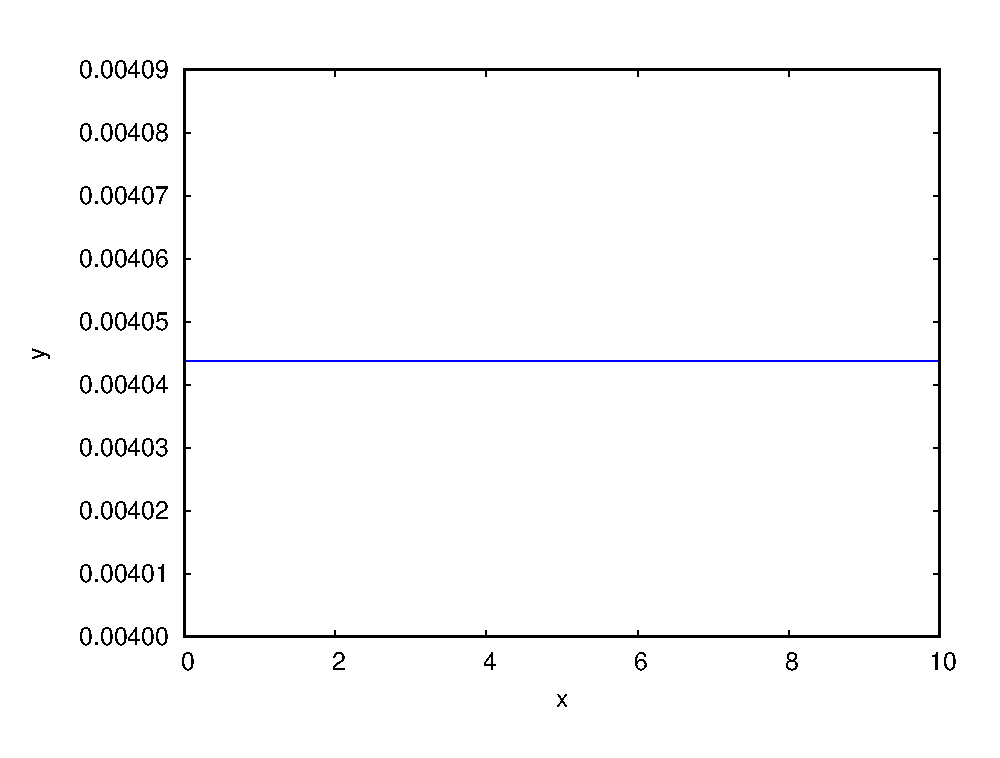
\includegraphics[width=\linewidth, height=30mm]{pic/_sol__0_0_1__0__10__1e2_kin_en}
    %     \caption{Кинетическая энергия}
    %     \label{fig:_sol__0_0_1__0__10__1e2_kin_en}
    % \end{subfigure}
    
    \begin{subfigure}[t]{0.3\textwidth}
        \centering
        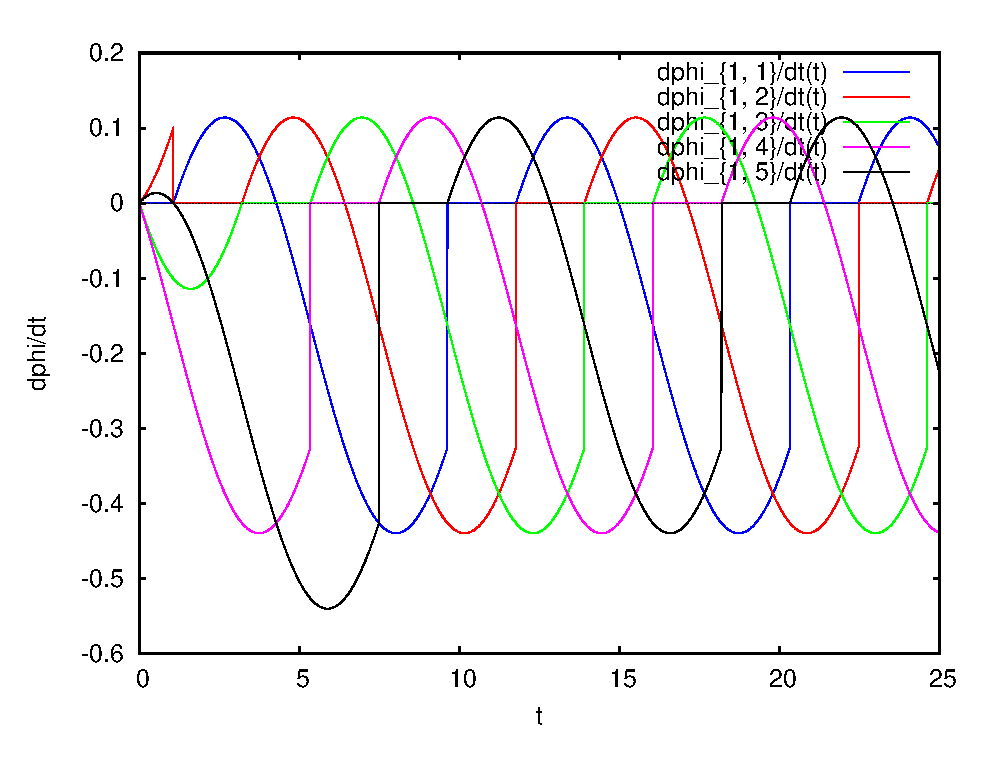
\includegraphics[width=\linewidth]{pic/rol__self_rot__velocities_of_rollers_of_wheel_1}
        \caption{Скорости роликов $\dot{\phi}_{ij}(t)$ на любом колесе}
        \label{fig:rol__self_rot__velocities_of_rollers_of_wheel_1}
    \end{subfigure}
    \begin{subfigure}[t]{0.3\textwidth}
        \centering
        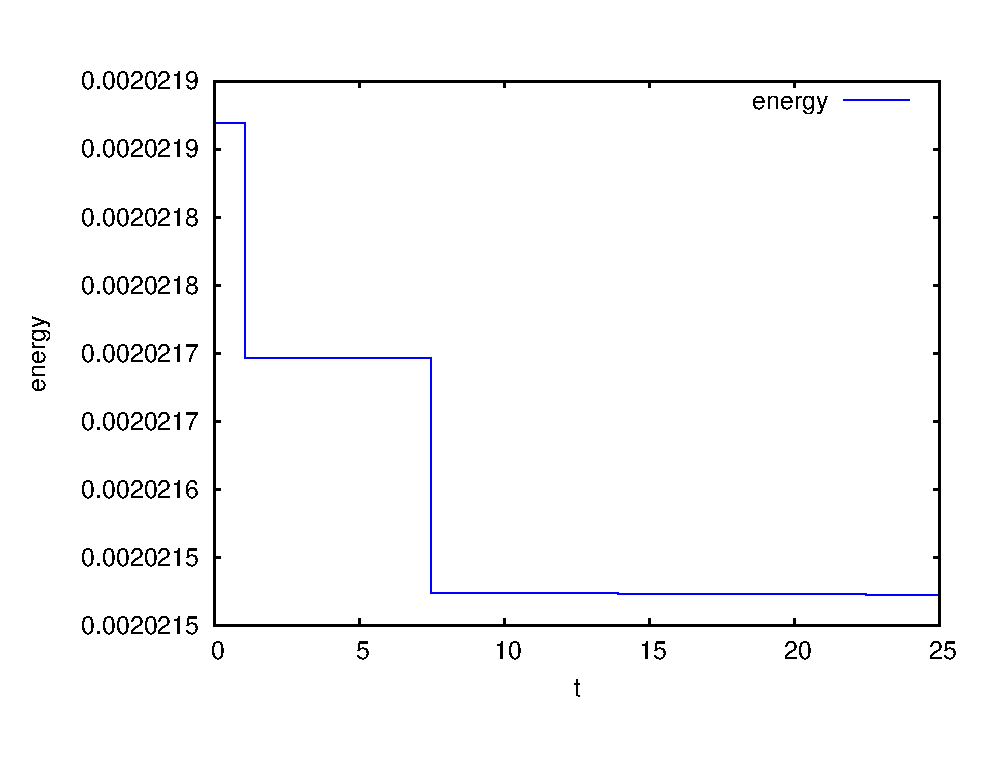
\includegraphics[width=\linewidth]{pic/rol__self_rot__kinetic_energy}
        \caption{Кинетическая энергия}
        \label{fig:rol__self_rot__kinetic_energy}    
    \end{subfigure}
    \begin{subfigure}[t]{0.3\textwidth}
        \centering
        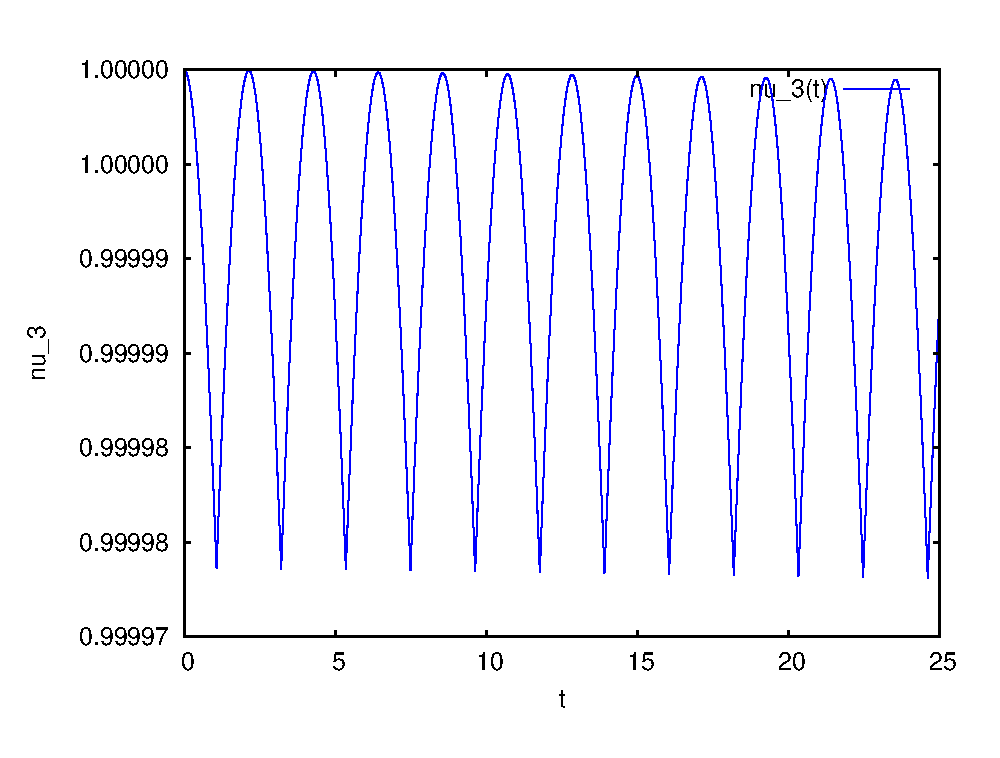
\includegraphics[width=\linewidth]{pic/rol__self_rot__velocity_of_self_rotation}
        \caption{Угловая скорость собственного вращения $\nu_3(t)$}
        \label{fig:rol__self_rot__velocity_of_self_rotation}    
    \end{subfigure}

    \caption{Экипаж с роликами. Вращение вокруг своей оси ($\nu_{1,2}(0) = 0, \nu_3 = 1$).}
    \label{fig:selfrot}
    
\end{figure}


% \begin{figure}
    \centering
    \begin{subfigure}[t]{0.3\textwidth}
        \centering
        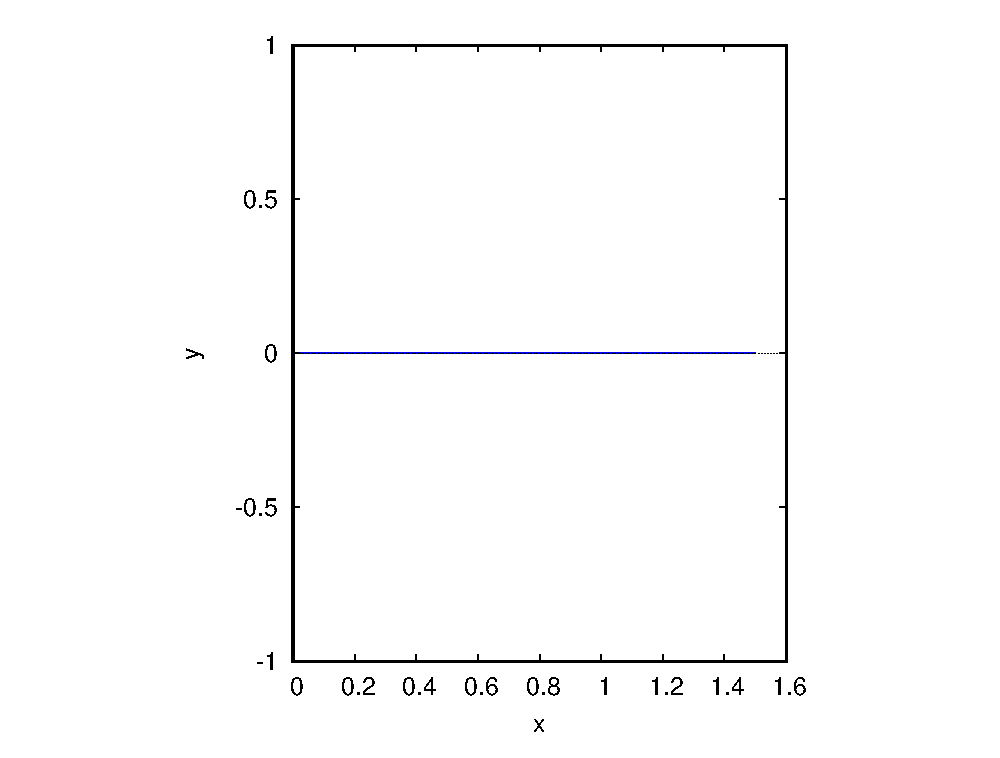
\includegraphics[width=\linewidth, height=30mm]{pic/_old_sol__1_0_0__0__10__1e2_trajectory}
        \caption{Траектория $X, Y$}
        \label{fig:_old_sol__1_0_0__0__10__1e2_trajectory}
    \end{subfigure}
    \begin{subfigure}[t]{0.3\textwidth}
        \centering
        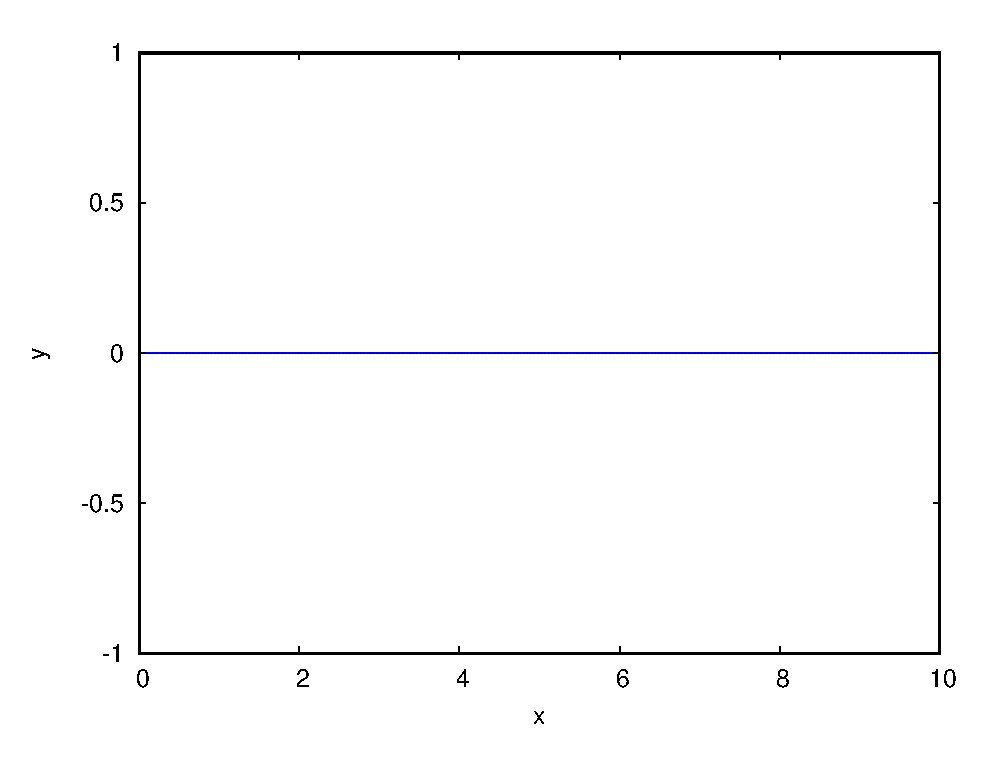
\includegraphics[width=\linewidth, height=30mm]{pic/_old_sol__1_0_0__0__10__1e2_theta}
        \caption{$\theta(t)$}
        \label{fig:_old_sol__1_0_0__0__10__1e2_theta}
    \end{subfigure}
    \vspace{12pt}
    
    \begin{subfigure}[t]{0.3\textwidth}
        \centering
        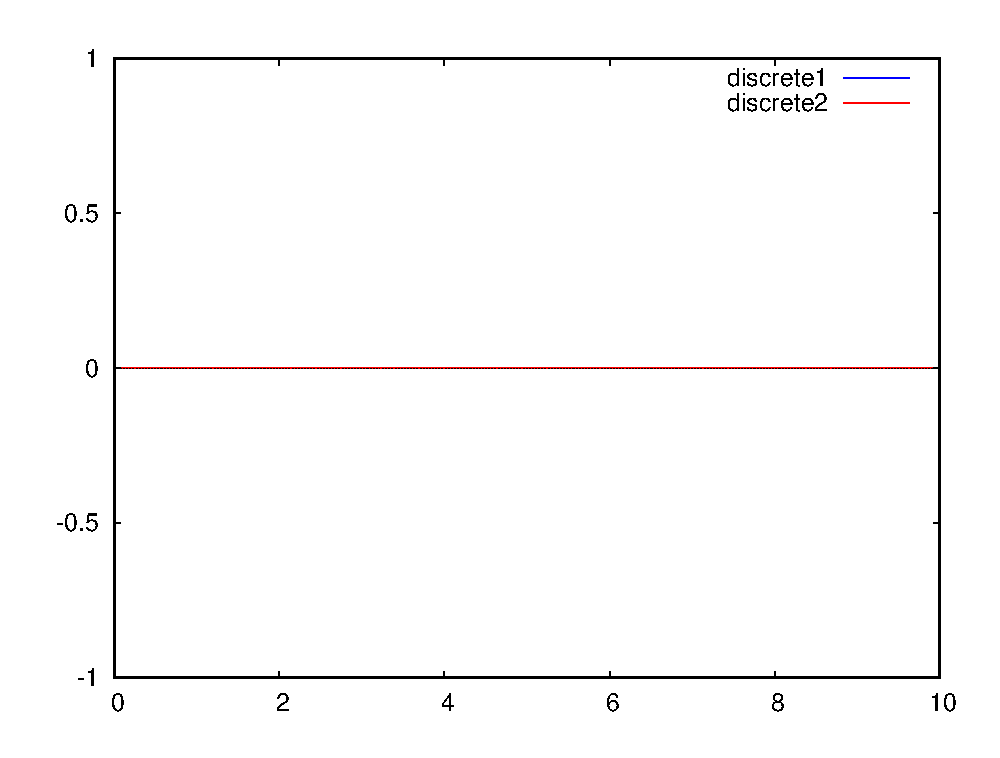
\includegraphics[width=\linewidth, height=30mm]{pic/_old_sol__1_0_0__0__10__1e2_nu12_centered}
        \caption{$\nu_1(t), \nu_2(t)$}
        \label{fig:_old_sol__1_0_0__0__10__1e2_nu12_centered}    
    \end{subfigure}
    \hfill
    \begin{subfigure}[t]{0.3\textwidth}
        \centering
        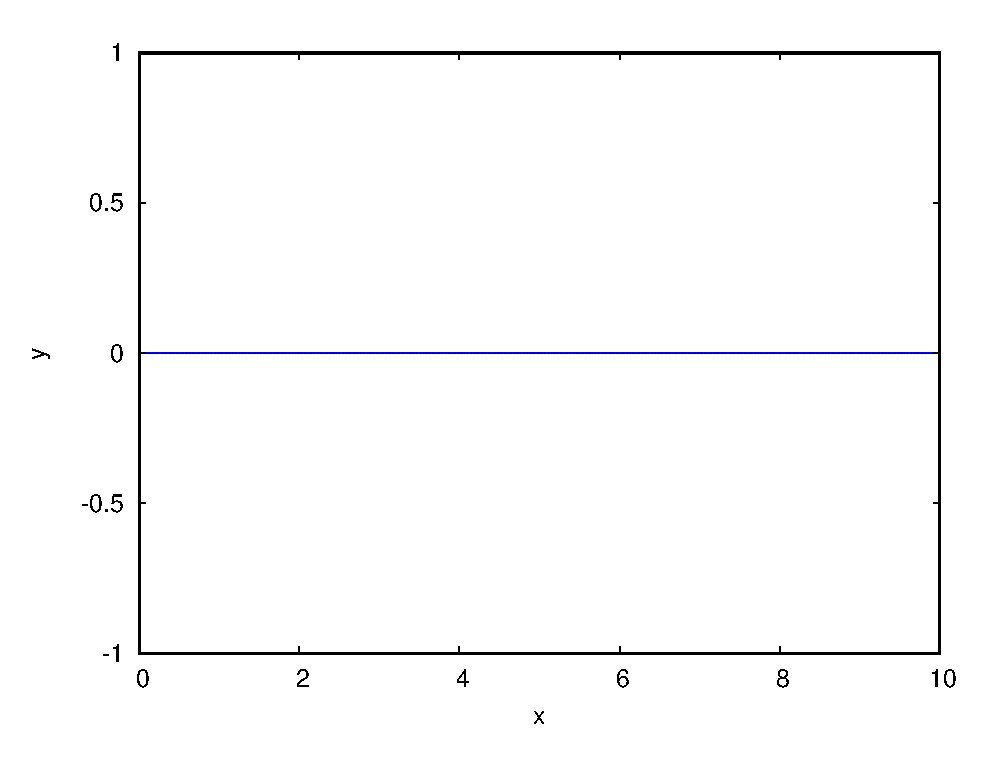
\includegraphics[width=\linewidth, height=30mm]{pic/_old_sol__1_0_0__0__10__1e2_nu3} \\
        \caption{$\nu_3(t)$}
        \label{fig:_old_sol__1_0_0__0__10__1e2_nu3}
    \end{subfigure}
    \hfill
    \begin{subfigure}[t]{0.3\textwidth}
        \centering
        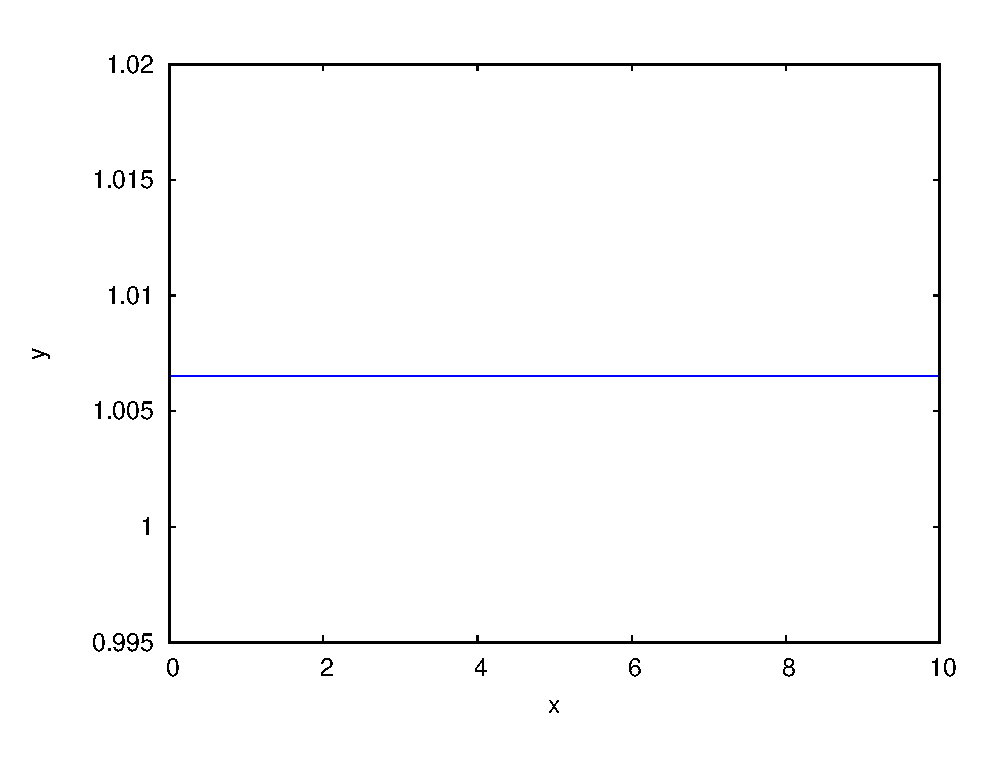
\includegraphics[width=\linewidth, height=30mm]{pic/_old_sol__1_0_0__0__10__1e2_kin_en}
        \caption{Кинетическая энергия}
        \label{fig:_old_sol__1_0_0__0__10__1e2_kin_en}
    \end{subfigure}
    
    \caption{Экипаж без роликов. Движение по прямой ($\nu_1(0) = 1, \nu_{2,3} = 0$). Экипаж равномерно движется по прямой, не вращаясь, энергия постоянна.}
    \label{fig:old_straight}
\end{figure}


% \begin{figure}[H]
    \centering

    \begin{columns}
        \column{0.45\textwidth}
            \centering
            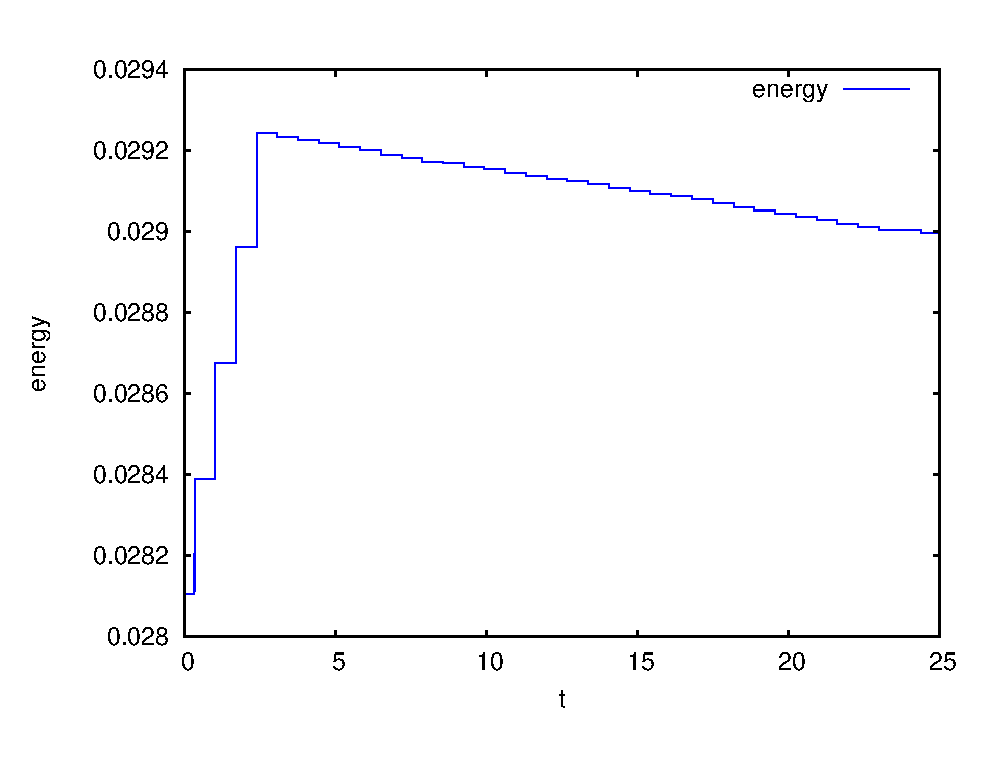
\includegraphics[width=\linewidth]{pic/rol__straight__kinetic_energy}\\
            Кинетическая энергия
        \column{0.45\textwidth}
            \centering
            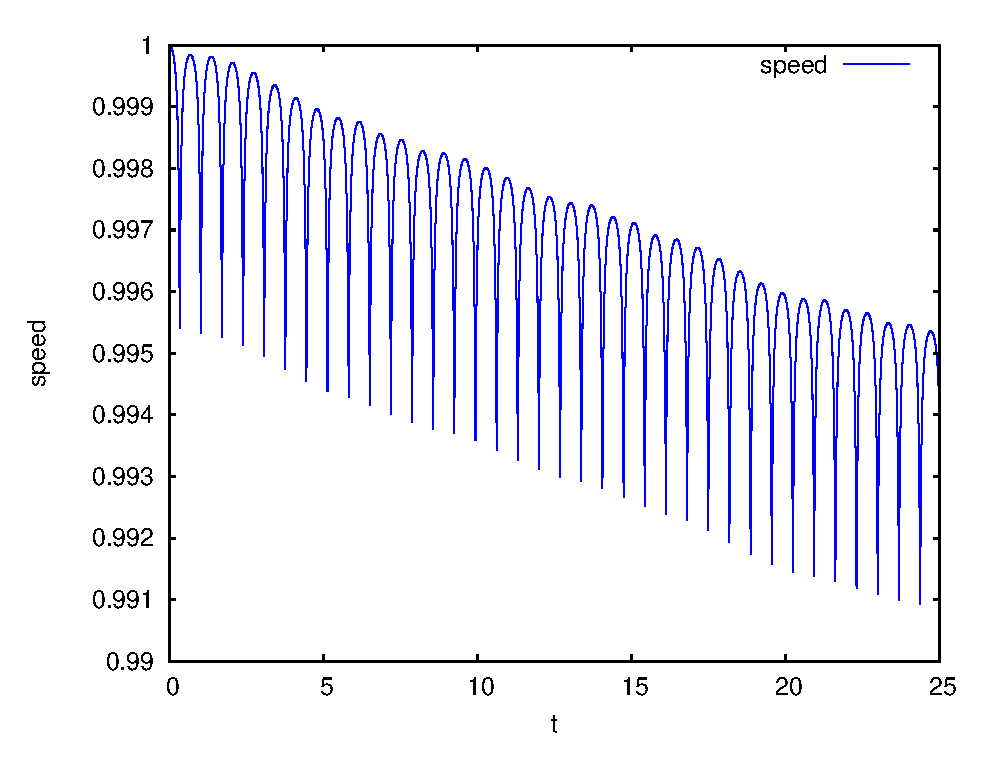
\includegraphics[width=\linewidth]{pic/rol__straight__speed_of_center_of_mass}\\
            Скорость центра масс
    \end{columns}
    
    \begin{columns}
        \column{0.35\textwidth}
            \centering
            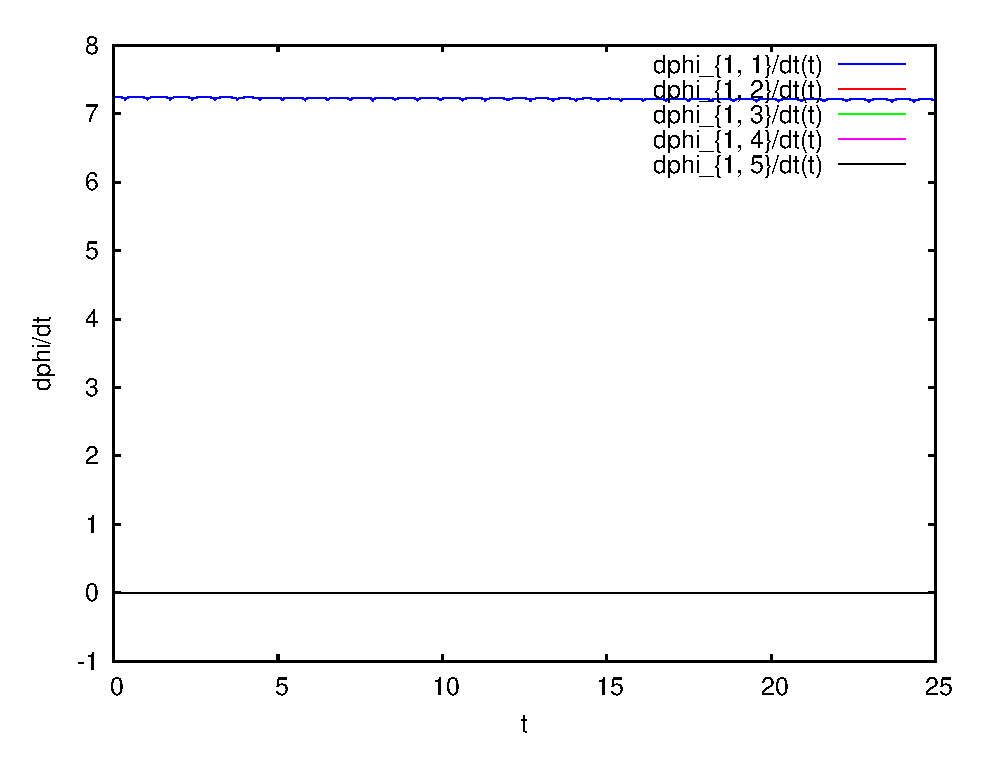
\includegraphics[width=\linewidth]{pic/rol__straight__velocities_of_rollers_of_wheel_1}\\
            $\dot{\phi}_{ij}(t)$ на переднем колесе
        \column{0.45\textwidth}
            \centering
            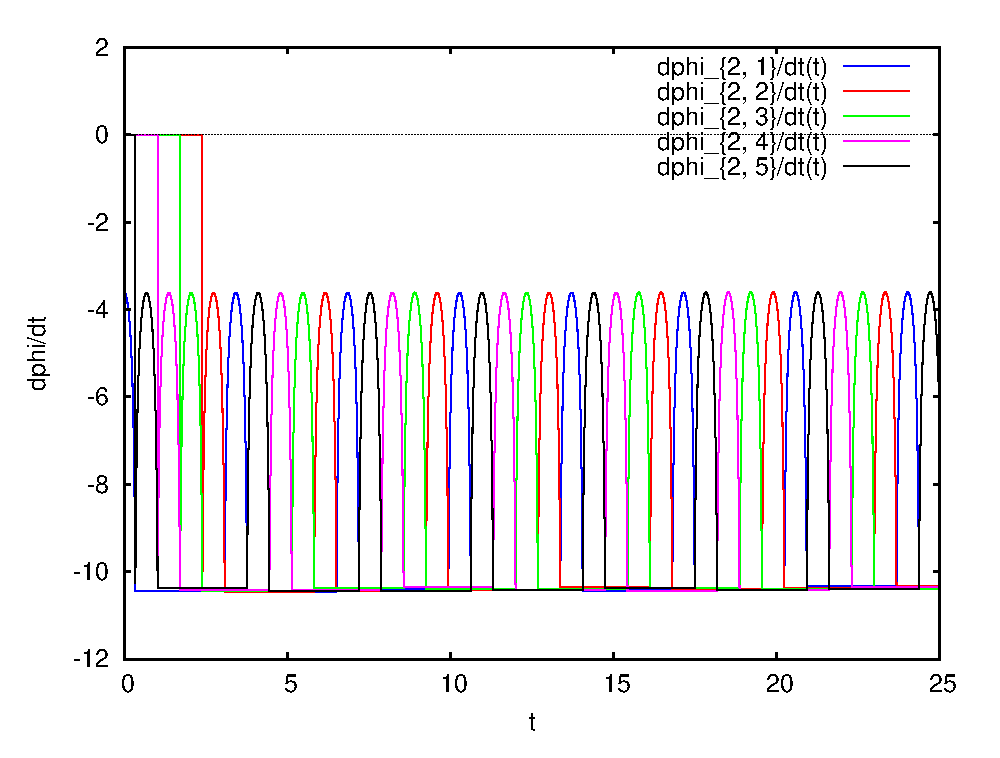
\includegraphics[width=\linewidth]{pic/rol__straight__velocities_of_rollers_of_wheel_2}\\
            $\dot{\phi}_{ij}(t)$ на правом заднем колесе
    \end{columns}

\end{figure}


%\section{Результаты расчетов}

{\bf Результаты расчетов.}
\stepcounter{section}

\begin{figure}
    \centering
    \begin{subfigure}[t]{0.3\textwidth}
        \centering
        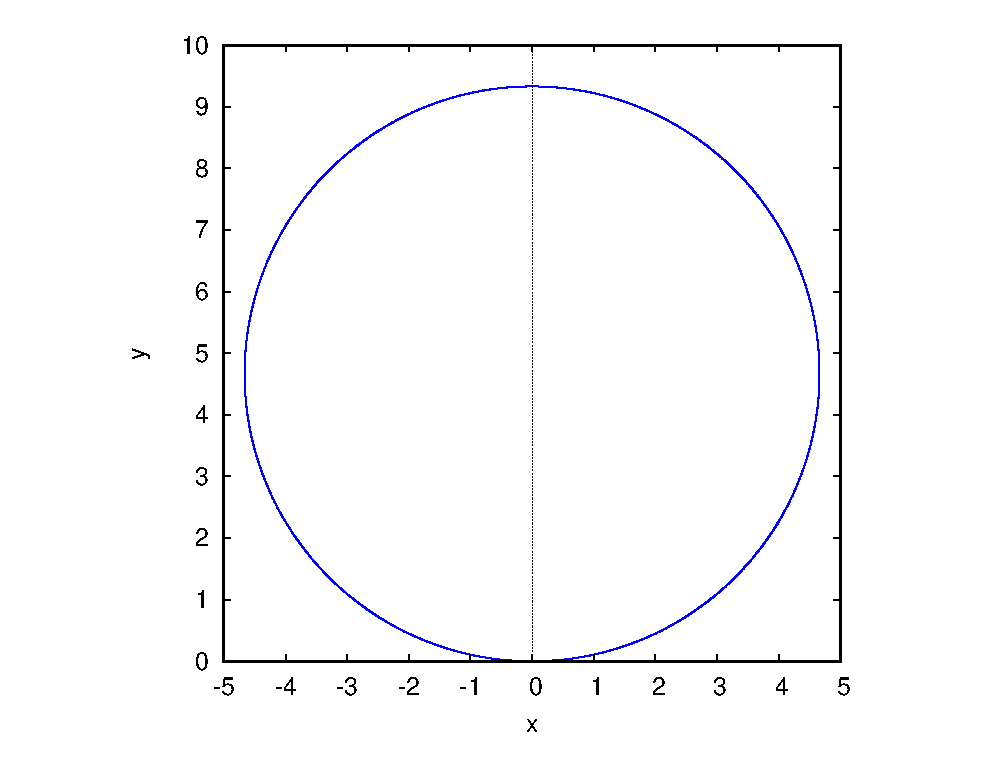
\includegraphics[width=\linewidth, height=30mm]{pic/_old_sol__1_0_1__0__230__1e2_trajectory}
        \caption{Траектория $X, Y$}
        \label{fig:_old_sol__1_0_1__0__230__1e2_trajectory}
    \end{subfigure}
    \begin{subfigure}[t]{0.3\textwidth}
        \centering
        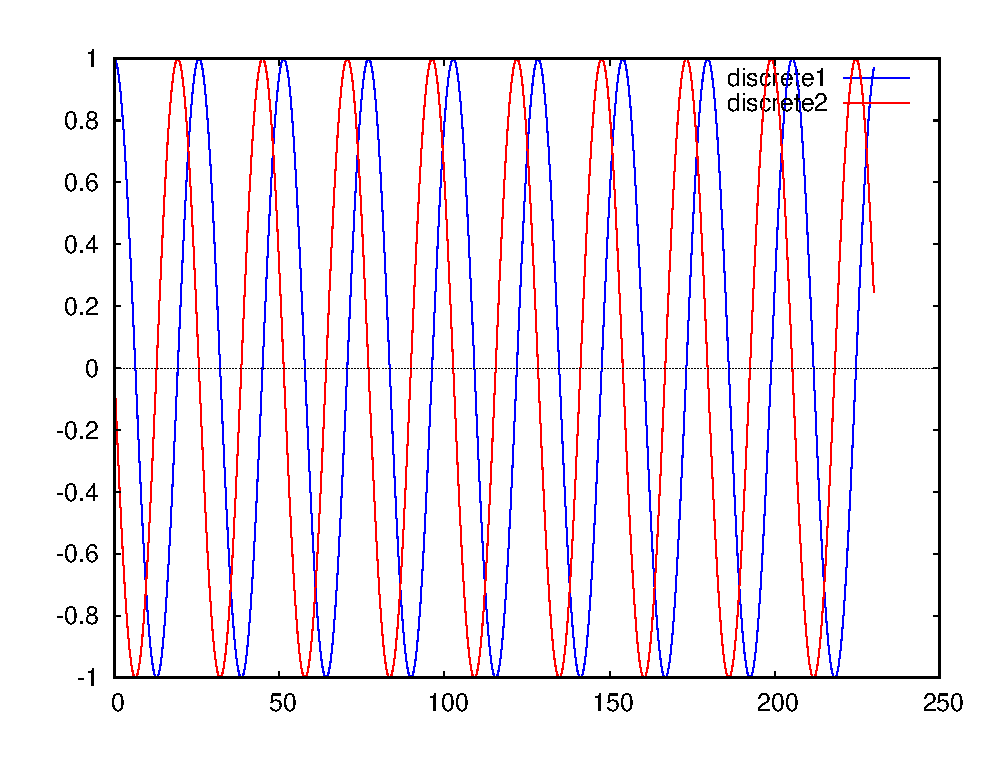
\includegraphics[width=\linewidth, height=30mm]{pic/_old_sol__1_0_1__0__230__1e2_nu12}
        \caption{$\nu_1(t), \nu_2(t)$}
        \label{fig:_old_sol__1_0_1__0__230__1e2_nu12}    
    \end{subfigure}
    % \begin{subfigure}[t]{0.3\textwidth}
    %     \centering
    %     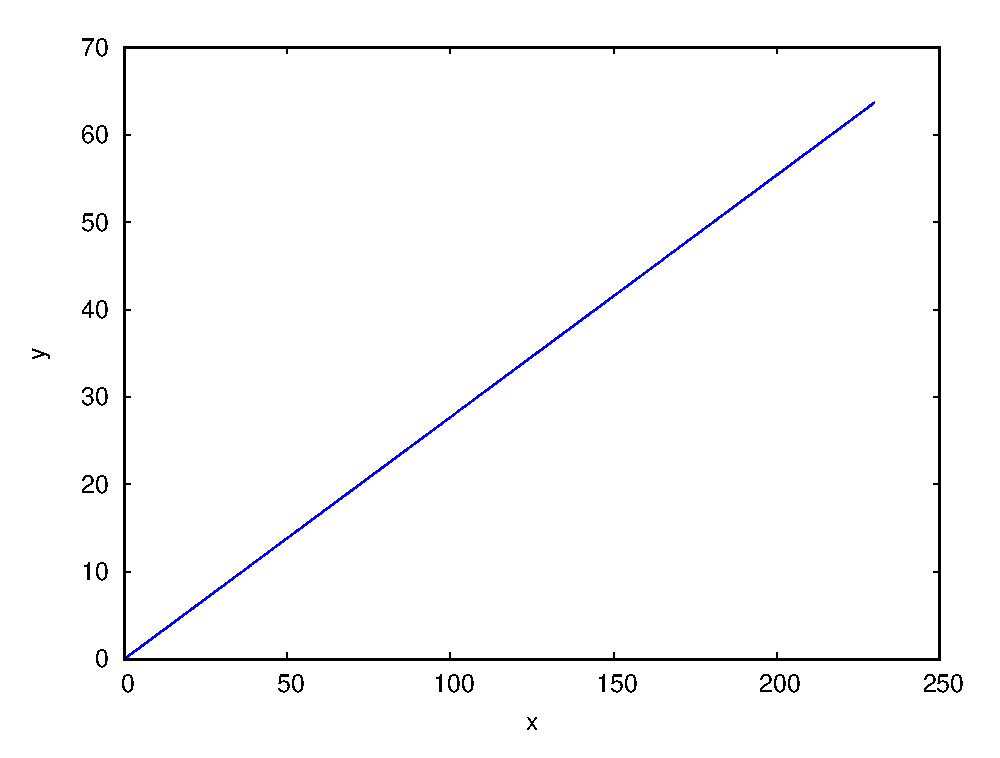
\includegraphics[width=\linewidth, height=30mm]{pic/_old_sol__1_0_1__0__230__1e2_theta}
    %     \caption{$\theta(t)$}
    %     \label{fig:_old_sol__1_0_1__0__230__1e2_theta}
    % \end{subfigure}
    % \vspace{12pt}
    
    % \begin{subfigure}[t]{0.3\textwidth}
    %     \centering
    %     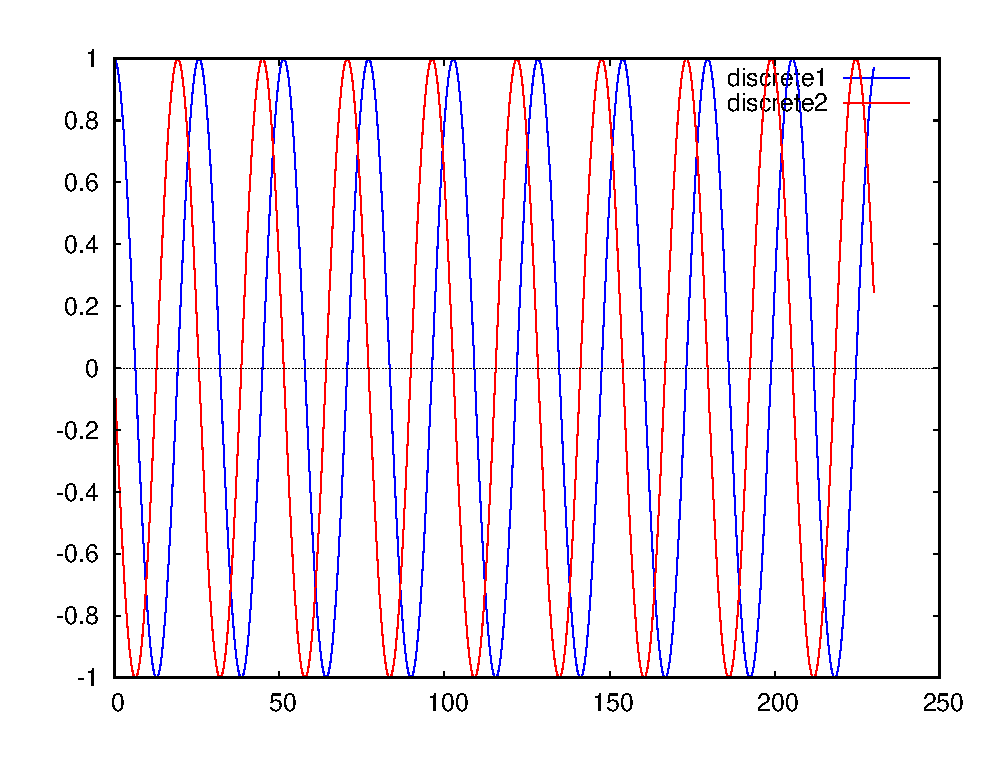
\includegraphics[width=\linewidth, height=30mm]{pic/_old_sol__1_0_1__0__230__1e2_nu12}
    %     \caption{$\nu_1(t), \nu_2(t)$}
    %     \label{fig:_old_sol__1_0_1__0__230__1e2_nu12}    
    % \end{subfigure}
    % \hfill
    % \begin{subfigure}[t]{0.3\textwidth}
    %     \centering
    %     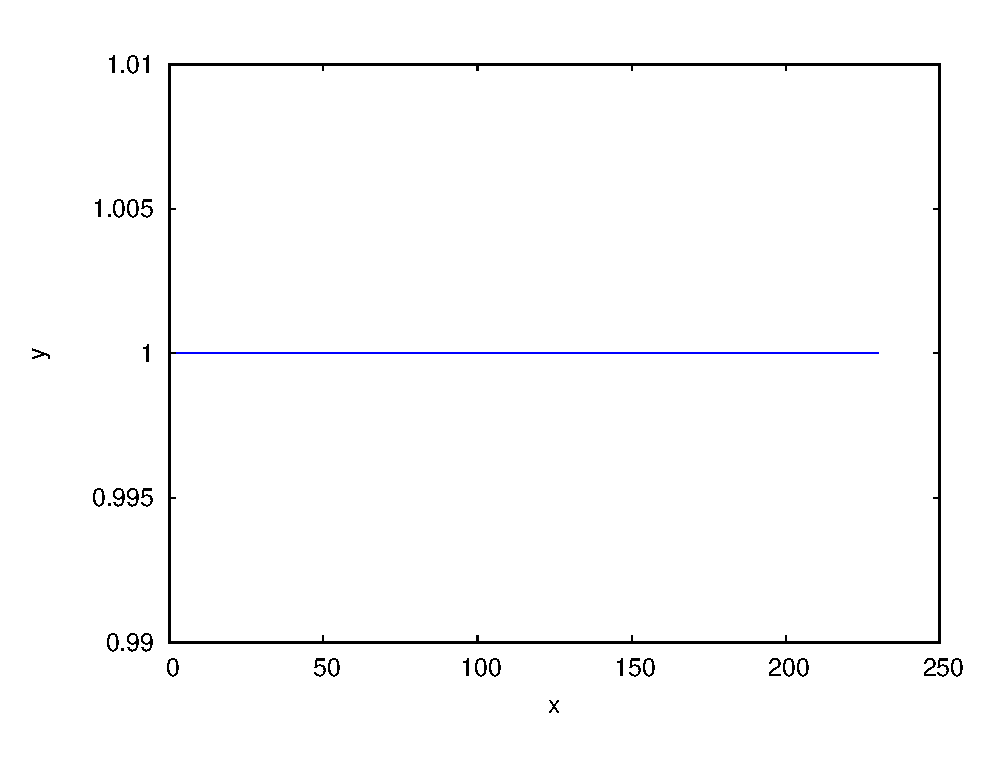
\includegraphics[width=\linewidth, height=30mm]{pic/_old_sol__1_0_1__0__230__1e2_nu3} \\
    %     \caption{$\nu_3(t)$}
    %     \label{fig:_old_sol__1_0_1__0__230__1e2_nu3}
    % \end{subfigure}
    % \hfill
    % \begin{subfigure}[t]{0.3\textwidth}
    %     \centering
    %     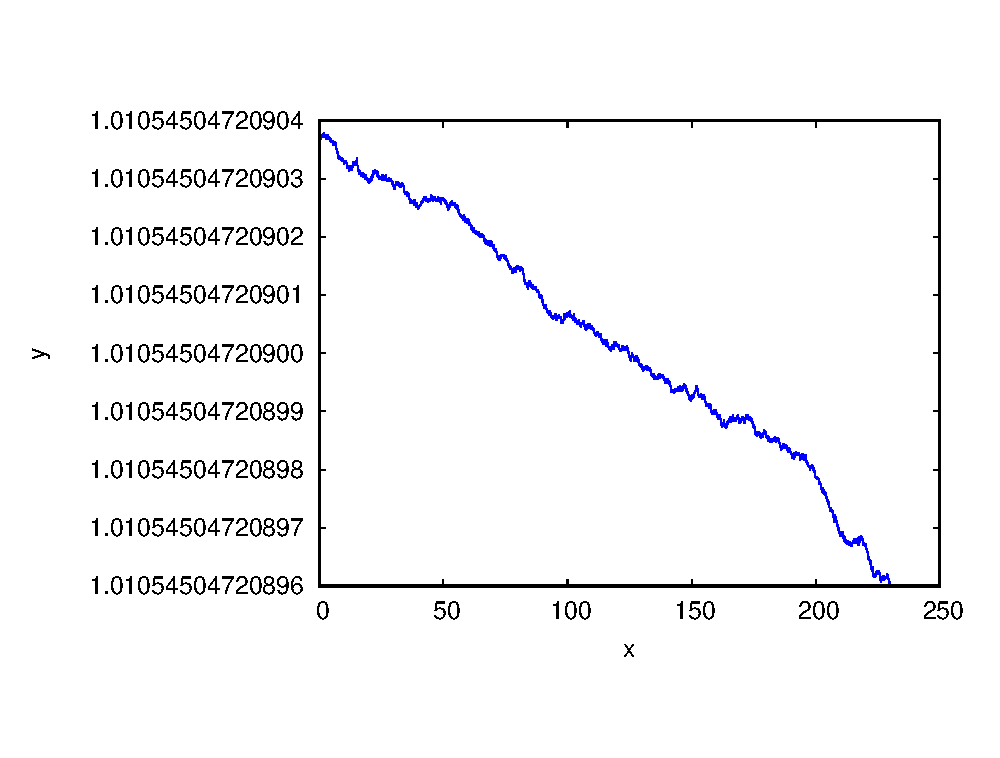
\includegraphics[width=\linewidth, height=30mm]{pic/_old_sol__1_0_1__0__230__1e2_kin_en}
    %     \caption{Кинетическая энергия}
    %     \label{fig:_old_sol__1_0_1__0__230__1e2_kin_en}
    % \end{subfigure}
    
    \caption{Экипаж без роликов. Движение с закруткой ($\nu_1(0) = 1, \nu_2(0) = 0, \nu_3(0) = 1$). Экипаж движется по окружности, равномерно вращаясь вокруг своей оси.}
    \label{fig:old_wrench}
\end{figure}


\begin{figure}
    \centering
    \begin{subfigure}[t]{0.45\textwidth}
        \centering
        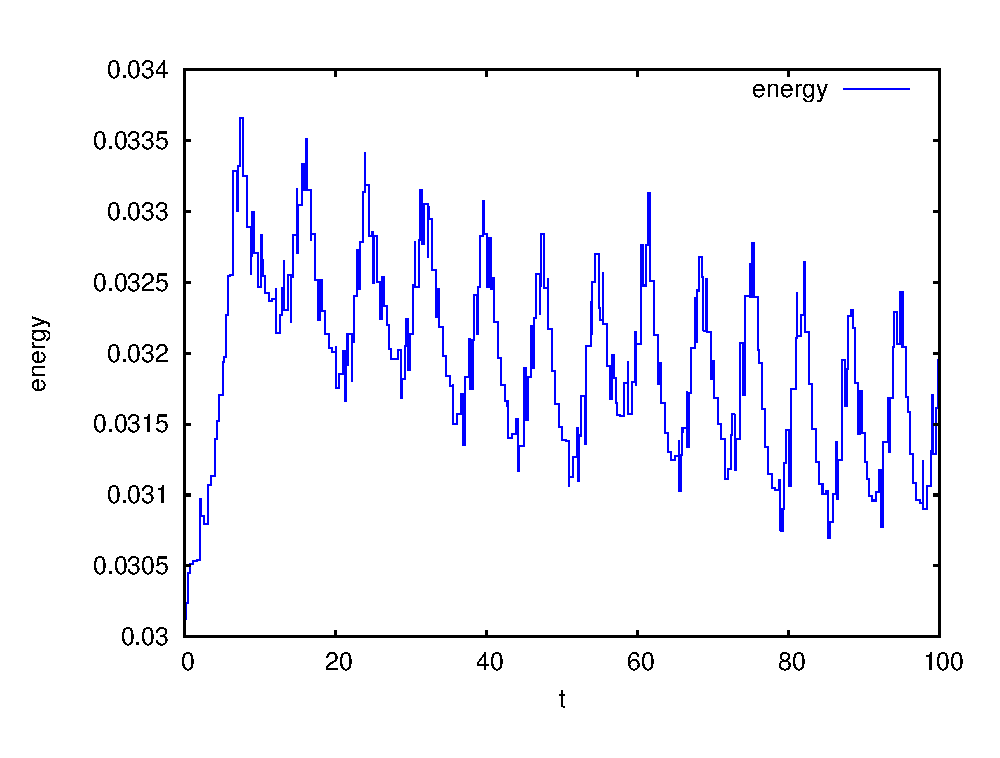
\includegraphics[width=\linewidth]{pic/rol__wrench__kinetic_energy}
        \caption{Кинетическая энергия}
        \label{fig:rol__wrench__kinetic_energy}
    \end{subfigure}
    \begin{subfigure}[t]{0.45\textwidth}
        \centering
        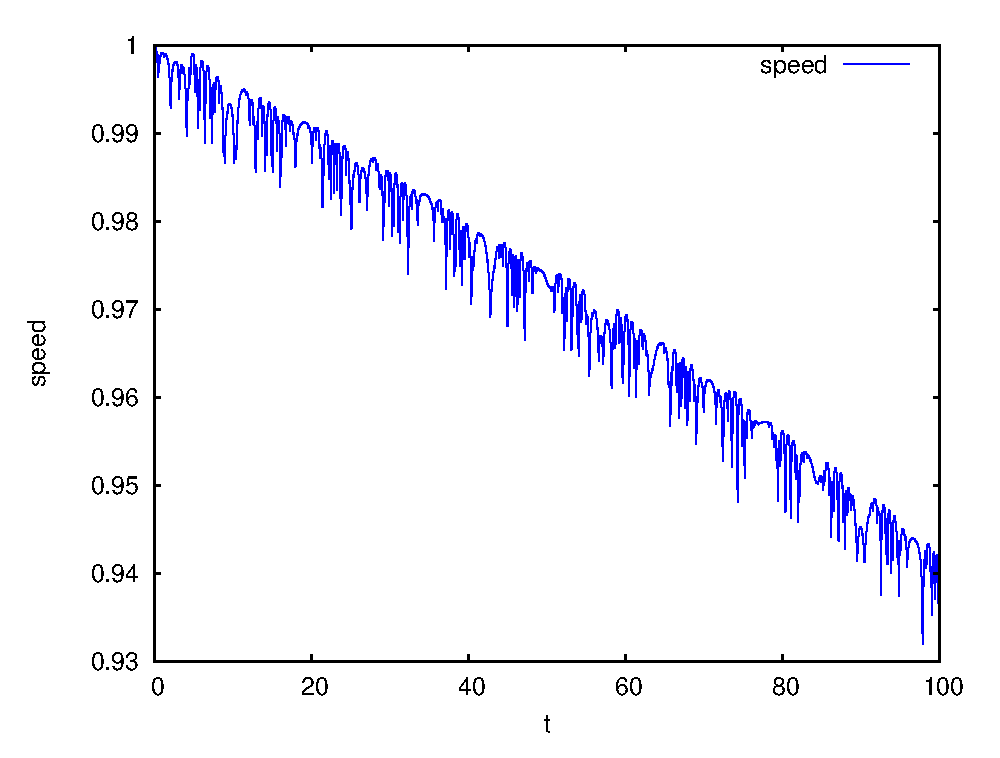
\includegraphics[width=\linewidth]{pic/rol__wrench__speed_of_center_of_mass}
        \caption{Скорость центра масс $\left(\nu_1^2 + \nu_2^2\right)(t)$}
        \label{fig:rol__wrench__speed_of_center_of_mass}
    \end{subfigure}
    \vspace{12pt}
    
    \begin{subfigure}[t]{0.45\textwidth}
        \centering
        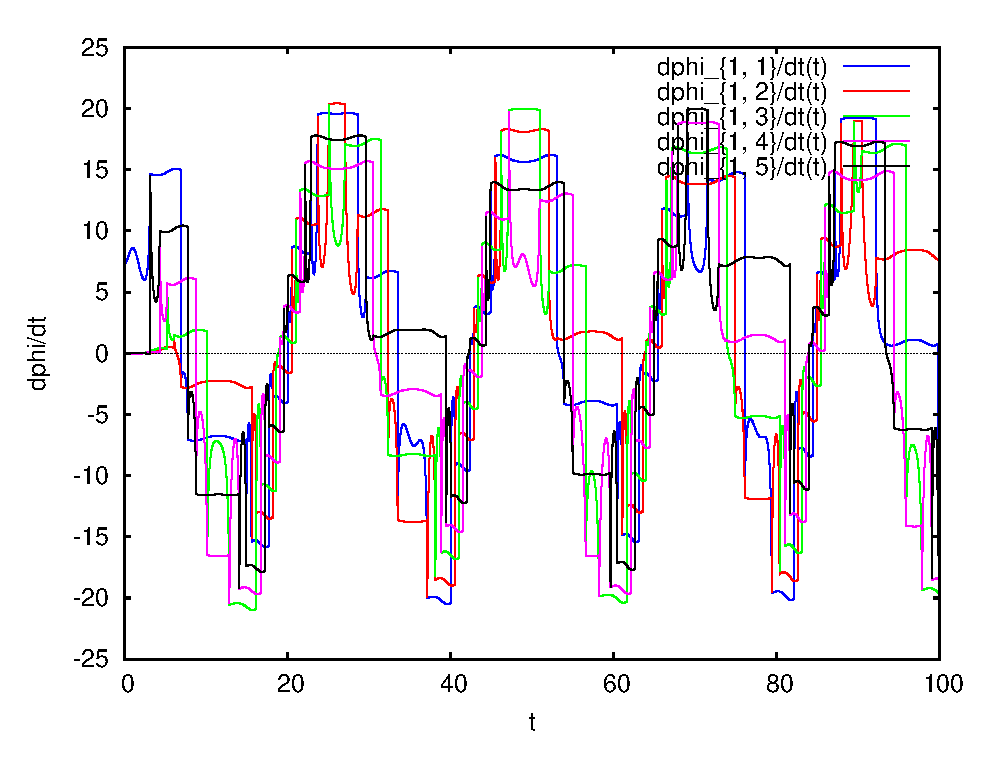
\includegraphics[width=\linewidth]{pic/rol__wrench__velocities_of_rollers_of_wheel_1}
        \caption{Скорости роликов $\dot{\phi}_{ij}(t)$ на первом колесе}
        \label{fig:rol__wrench__velocities_of_rollers_of_wheel_1}    
    \end{subfigure}
    \hfill
    \begin{subfigure}[t]{0.45\textwidth}
        \centering
        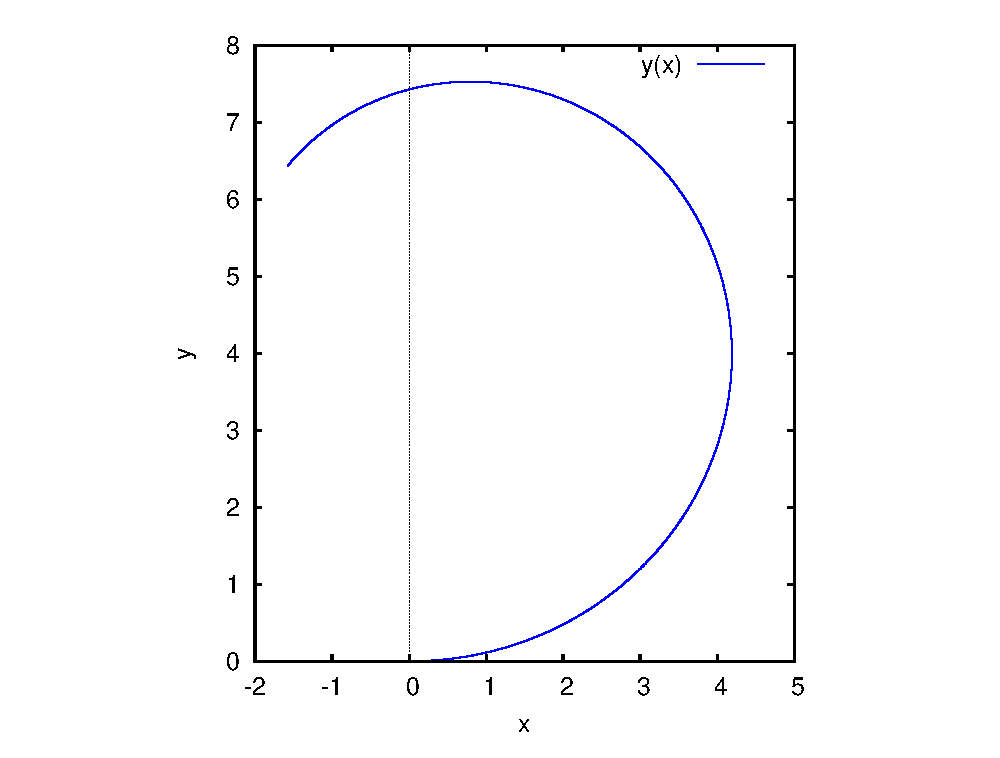
\includegraphics[width=\linewidth]{pic/rol__wrench__trajectory} \\
        \caption{Траектория центра масс на плоскости $OXY$}
        \label{fig:rol__wrench__trajectory}
    \end{subfigure}
    
    \caption{Экипаж c роликами. Движение с закруткой ($\nu_1(0) = 1, \nu_2(0) = 0, \nu_3(0) = 1$).}
    \label{fig:wrench}
    
\end{figure}


\begin{figure}
    \centering
    \begin{subfigure}[t]{0.3\textwidth}
        \centering
        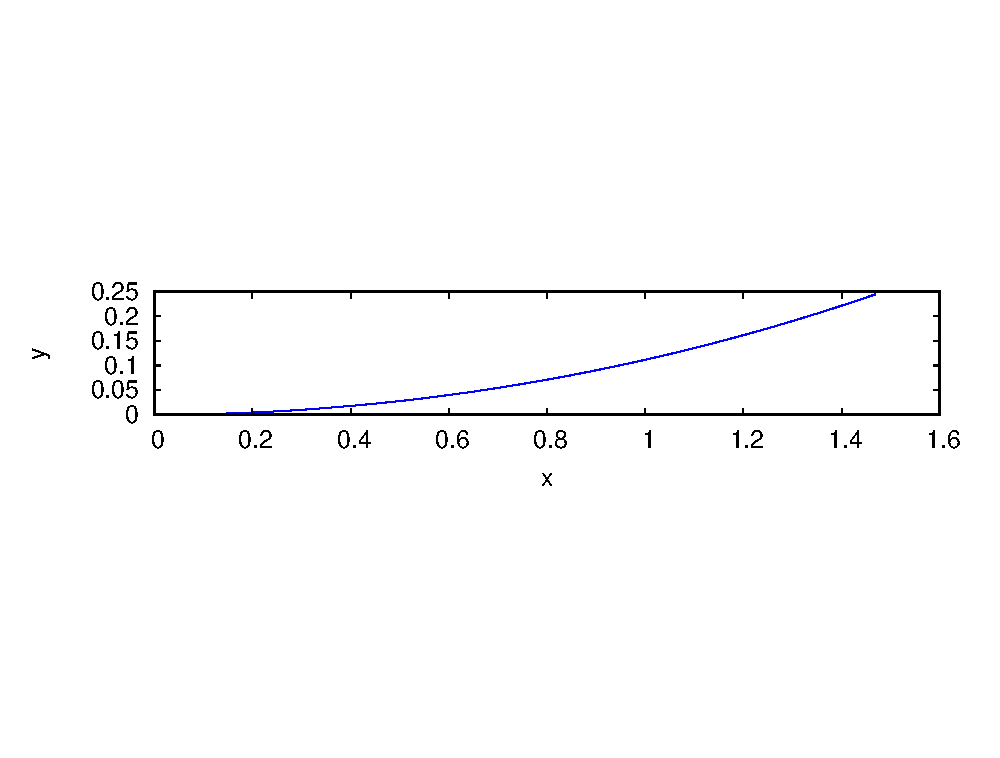
\includegraphics[width=\linewidth, height=30mm]{pic/_sol__1_0_1__0__10__1e2_trajectory}
        \caption{Траектория $X, Y$}
        \label{fig:_sol__1_0_1__0__10__1e2_trajectory}
    \end{subfigure}
    \begin{subfigure}[t]{0.3\textwidth}
        \centering
        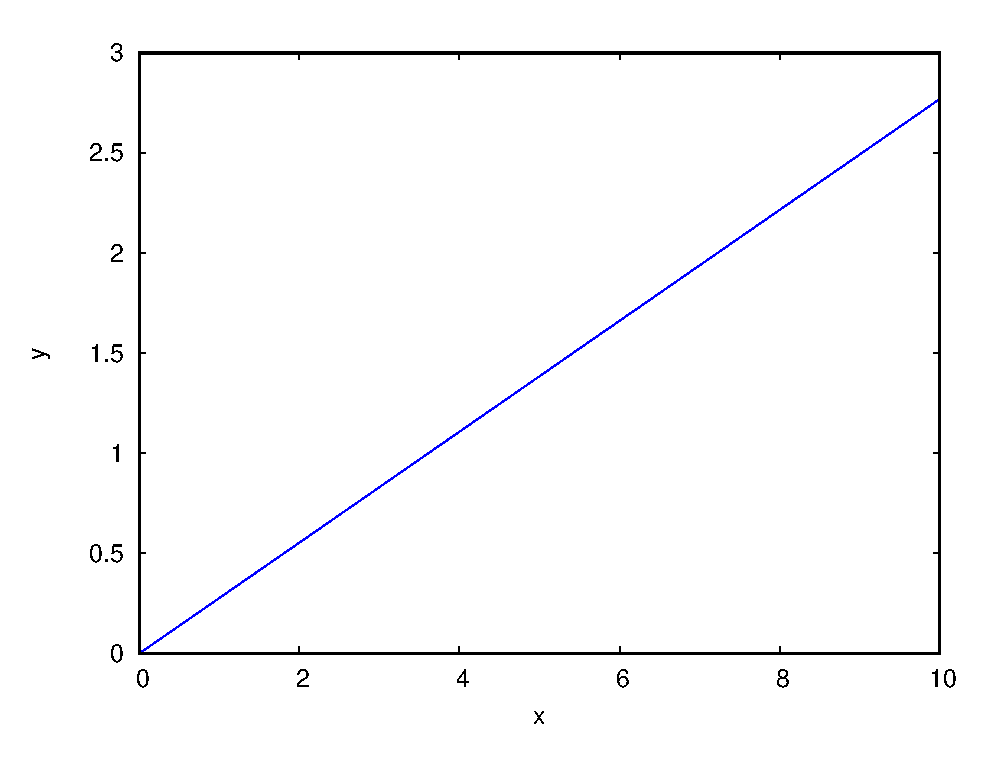
\includegraphics[width=\linewidth, height=30mm]{pic/_sol__1_0_1__0__10__1e2_theta}
        \caption{$\theta(t)$}
        \label{fig:_sol__1_0_1__0__10__1e2_theta}
    \end{subfigure}
    \vspace{12pt}
    
    \begin{subfigure}[t]{0.3\textwidth}
        \centering
        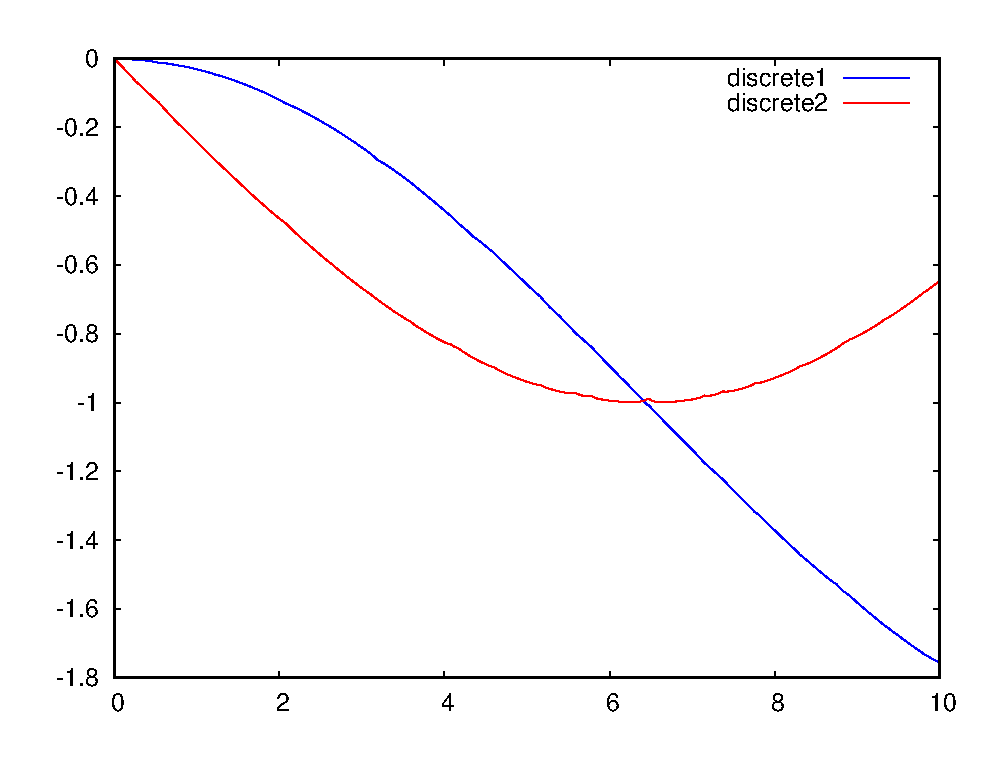
\includegraphics[width=\linewidth, height=30mm]{pic/_sol__1_0_1__0__10__1e2_nu12_centered}
        \caption{$\nu_1(t), \nu_2(t)$}
        \label{fig:_sol__1_0_1__0__10__1e2_nu12_centered}    
    \end{subfigure}
    \hfill
    \begin{subfigure}[t]{0.3\textwidth}
        \centering
        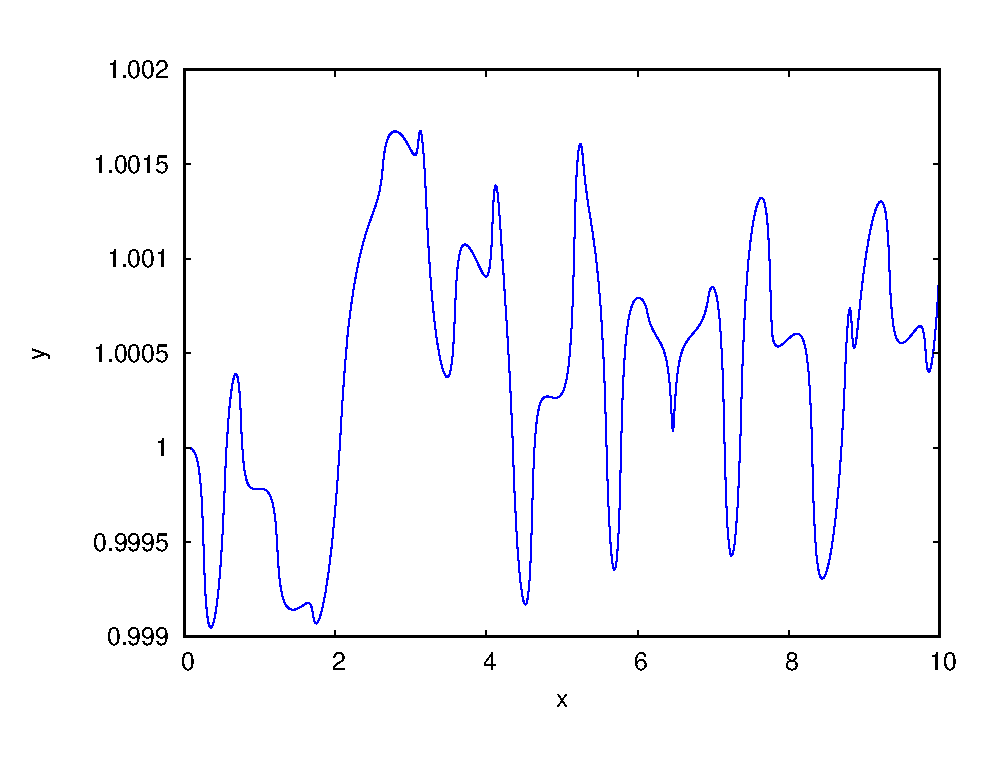
\includegraphics[width=\linewidth, height=30mm]{pic/_sol__1_0_1__0__10__1e2_nu3} \\
        \caption{$\nu_3(t)$}
        \label{fig:_sol__1_0_1__0__10__1e2_nu3}
    \end{subfigure}
    \hfill
    \begin{subfigure}[t]{0.3\textwidth}
        \centering
        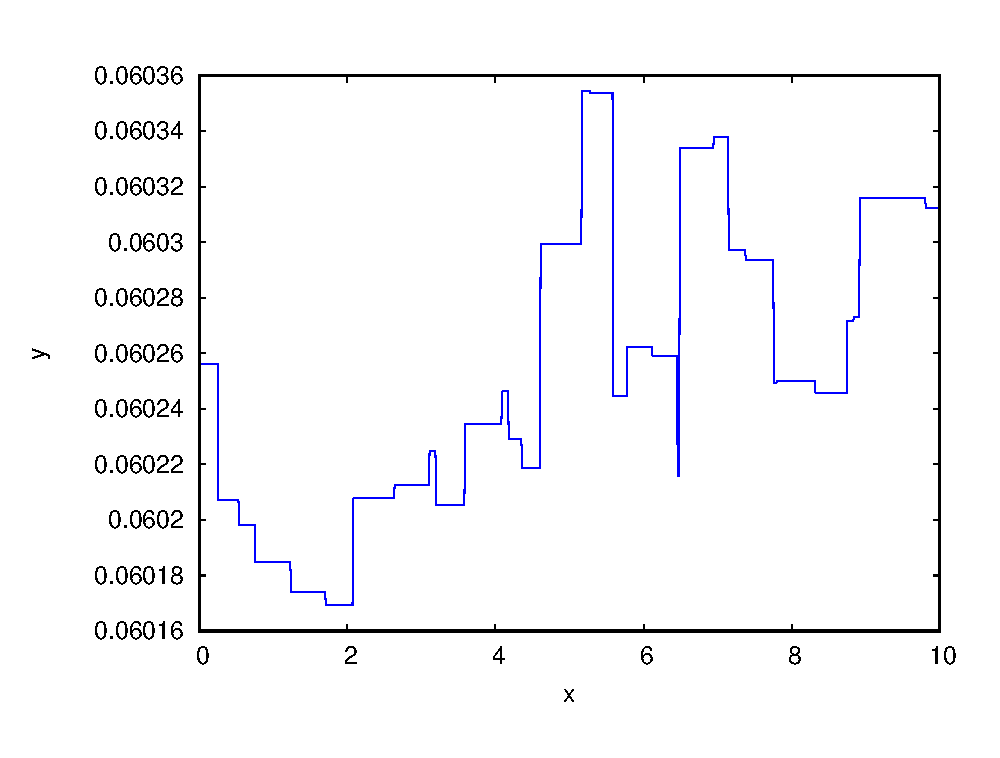
\includegraphics[width=\linewidth, height=30mm]{pic/_sol__1_0_1__0__10__1e2_kin_en}
        \caption{Кинетическая энергия}
        \label{fig:_sol__1_0_1__0__10__1e2_kin_en}
    \end{subfigure}
    
    \caption{Экипаж c роликами. Движение с закруткой ($\nu_1(0) = 1, \nu_2(0) = 0, \nu_3(0) = 1$) на коротком промежутке времени. Псевдоскорости не постоянны, виден ступенчатый вид кинетической энергии.}
    \label{fig:wrench_short}
\end{figure}


\section{Выводы}

Получены уравнения движения экипажа с полным набором роликов в неголономной постановке.

Показано, что разница с уравнениями для системы без роликов пропорциональна моменту инерции ролика.

Предложена модель перехода с ролика на ролик.

Получены численные решения при неподвижных свободных роликах для симметричной конфигурации.


% BibTeX users please use one of
%\bibliographystyle{spbasic}      % basic style, author-year citations
\bibliographystyle{./springer/spmpsci}      % mathematics and physical sciences
%\bibliographystyle{spphys}       % APS-like style for physics
\bibliography{omni}   % name your BibTeX data base

\end{document}


